\documentclass[12pt,a4paper,twoside,titlepage]{book}

% inclusione librerie
% NB: il pacchetto hyperref va caricato per ultimo ma prima del pacchetto 
% glossaries altrimenti l'indice del PDF non viene generato correttamente!
\usepackage[italian]{babel}
\usepackage{tikz}
\usepackage{graphicx}
\usepackage{frontespizio}
\usepackage[Lenny]{fncychap}
\usepackage{longtable}
\usepackage{minted}
\usepackage{pgf-umlsd}
\usepackage[bookmarks]{hyperref}
\usepackage[acronyms]{glossaries}

% impostazione interlinea
\linespread{1.2}

% configurazione tikz
\usetikzlibrary{automata, positioning, arrows, shapes}
\tikzset{->, >=stealth', node distance=5cm, initial text=$ $}

% configurazione minted
\setminted{
    frame=lines,
    framesep=2mm,
    baselinestretch=1.2,
    fontsize=\footnotesize,
    linenos
}

% necessario per far funzionare il pacchetto per glossari/acronimi
\makeglossaries

% acronimi
\newacronym{iot}{IoT}{Internet of Things}
\newacronym{aws}{AWS}{Amazon Web Services}
\newacronym[\glslongpluralkey={Radiatori Elettrici}, \glsshortpluralkey=RE]{re}{RE}{Radiatore Elettrico}
\newacronym{gpio}{GPIO}{General Purpose Input Output}
\newacronym{adc}{ADC}{Analog to Digital Converter}
\newacronym{mcu}{MCU}{Micro Controller Unit}
\newacronym{uart}{UART}{Universal Asyncronous Receive and Transmit}
\newacronym{tls}{TLS}{Transport Layer Security}
\newacronym{usb}{USB}{Universal Serial Bus}
\newacronym{rf}{RF}{Radio Frequenza}
\newacronym{ota}{OTA}{Over The Air update}
\newacronym{hmi}{HMI}{Human Machine Interface}
\newacronym{ble}{BLE}{Bluetooth Low Energy}
\newacronym{http}{HTTP}{Hyper Text Transfer Protocol}
\newacronym{spi}{SPI}{Serial Peripherial Interface}
\newacronym{ci}{CI}{Continuos Integration}
\newacronym{cd}{CD}{Continuos Delivery}
\newacronym{vmc}{VMC}{Ventilazione Meccanica Controllata}
\newacronym{rgbw}{RGBW}{Red Green Blue White}
\newacronym{ntc}{NTC}{Negative Temperature Coefficient}
\newacronym{led}{LED}{Light Emitting Diode}
\newacronym{rtos}{RTOS}{Real Time Operating System}
\newacronym{rtc}{RTC}{Real Time Clock}
\newacronym{ap}{AP}{Access Point}
\newacronym{sta}{STA}{Station}
\newacronym{pwm}{PWM}{Pulse Width Modulation}
\newacronym{sdk}{SDK}{Software Development Kit}
\newacronym{yat}{YAT}{Yet Another Thermostat}
\newacronym{cu}{CU}{Connection Unit}
\newacronym{red}{RED}{Radio Equipment Device}
\newacronym{emc}{EMC}{Electro Magnetic Compliance}
\newacronym{bt}{BT}{Bassa Tensione}
\newacronym{sil}{SIL}{System Integrity Level}
\newacronym{ca}{CA}{Certification Authority}
\newacronym{json}{JSON}{JavaScript Object Notation}

% glossario
\newglossaryentry{mqtt}{
    name=MQTT,
    description={Protocollo di scambio di messaggi di tipo publish/subscribe pensato 
        per l'utilizzo su dispositivi con scarse risorse hardware, quali ad esempio 
        i dispositivi \acrshort{iot}}
}

\newglossaryentry{micro}{
    name=microcontrollore,
    description={Componente elettronico che integra in un unico chip processore, memoria
        RAM, memoria flash, gestione delle periferiche di input/output \acrshort{gpio}. Tipicamente offre 
        prestazioni molto limitate ma bassi costi e bassi consumi energetici}
}

\newglossaryentry{firmware}{
    name=firmware,
    description={La componente software che viene eseguita su un dispositivo embedded}
}

\newglossaryentry{wifi}{
    name=Wi-Fi,
    description={Protocollo radio che consente la comunicazione su rete TCP/IP senza cavi}
}

\newglossaryentry{gateway}{
    name=gateway,
    description={Dispositivo hardware che mette in comunicazione due reti di tipologie differenti,
        ad esempio una rete TCP/IP e dispositivi \acrshort{rf}}
}

\newglossaryentry{cloud}{
    name=cloud,
    description={Insieme di tecnolgoie che permettono di archiviare ed elaborare i dati in rete, anziché 
        su un dispositivo locale}
}

\newglossaryentry{serverless}{
    name=serverless,
    description={Modello di sviluppo \gls{cloud} che consente di creare ed eseguire 
        applicazioni in rete senza doversi preoccupare della gestione dei server. Tipicamente il sistema 
        scala in maniera automatica, andando a creare/eliminare risorse in base al carico del sistema}
}

\newglossaryentry{topic}{
    name={topic MQTT},
    description={Stringa testuale che identifica un canale di comunicazione sul quale un client \Gls{mqtt}
        può inviare o ricevere messaggi}
}

\newglossaryentry{broker}{
    name={broker MQTT},
    description={Componente server del protocollo \Gls{mqtt} che si occupa di instradare i messaggi pubblicati 
        dai client ad essi connessi ad altri client a seconda dei \gls{topic} ai quali si sono sottoscritti}
}

\newglossaryentry{awsjob}{
    name={Job IoT Core},
    description={Sistema di distribuzione di processi batch da eseguire sui dispositivi collegati ad \Gls{iotcore}. 
        Ogni processo è identificato da un documento \acrshort{json}, a libera scelta di chi lo crea, che il dispositivo interpreta 
        per ottenere l'operazione da effettuare. Il dispositivo aggiorna lo stato di esecuzione del processo batch 
        in AWS IoT Core, ed AWS IoT Core permette di settare delle logiche di distribuzione graduali del processo 
        (ad esempio annulla se il job fallisce in più del 5\% dei dispositivi, ecc). }
}

\newglossaryentry{iotcore}{
    name={IoT Core},
    description={Servizio \gls{serverless} di \gls{broker} gestito da \Gls{aws}}
}

\newglossaryentry{git}{
    name={Git},
    description={Sistema di controllo versione del codice sorgente gestito distribuito. Creato inizialmente da Linus 
        Torvalds per l'uso in Linux, è ad oggi il sistema più utilizzato ed evoluto sul mercato}
}

\newglossaryentry{now}{
    name={``IRSAP NOW''},
    description={Piattaforma di termoregolazione cloud dell'azienda IRSAP s.p.a. Consente di gestire attraverso 
        un'unica app iOS/Android tutti i dispositivi di termoregolazione connessi del catalogo IRSAP, quali 
        radiatori elettrici, impianti idraulici e sistemi \acrshort{vmc}}
}

\newglossaryentry{i2c}{
    name=i2c,
    description={Protocollo di comunicazione seriale su due segnali elettrici (SDA ed SCL) per la comunicazione 
        fra chip embedded, quali microcontrollori e sensori}
}

\newglossaryentry{arm}{
    name=ARM,
    description={Architettura hardware RISC sviluppata dall'azienda ARM. La sua versione Core M è particolarmente 
        utilizzata all'interno di processore embedded low-power.}
}

\newglossaryentry{filpilote}{
    name={Fil Pilote},
    description={Standard francese per il comando di radiatori elettrici in maniera centralizzata. Consiste in un 
        secondo cavo in cui in base alla modalità arriva un segnale a 230V AC che codifica 4 modalità di funzionamento:
        COMFORT (assenza di segnale), ECO (segnale 230AC completo), OFF (solo componente positiva della sinusoide 230V), 
        ANTIGELO (solo componente negativa della sinusoide 230V)}
}

\newglossaryentry{modbus}{
    name=Modbus,
    description={Protocollo di comunicazione master/slave fra dispositivi embedded. Può funzionare sia su interfaccia 
        fisica seriale \acrshort{uart} che su stack di rete TCP/IP}
}

\newglossaryentry{opentherm}{
    name=OpenTherm,
    description={Protocollo standard definito dal consorzio OpenTherm per la comunicazione fra termostati e generatori 
        di calore (principalmente caldaie). È un protocollo master/slave dove il master è il termostato ambiente (o una 
        centralina di controllo) e lo slave il generatore di calore. L'interfaccia fisica è un bus composto da due cavi 
        che è in grado oltre a portare i dati di fornire alimentazione al dispositivo master (termostato).}
}

% macro
\newcommand*{\fullref}[1]{\hyperref[{#1}]{\nameref*{#1} (\ref*{#1})}}

% fine preambolo

\begin{document}

% inizio parte iniziale (numeri romani)
% nota che deve essere prima del frontespizio per far funzionare correttamente i link!
\frontmatter

% pagina del titolo
\begin{frontespizio}
    \Universita{Verona}
    \Dipartimento{Scienze e ingegneria}
    \Corso{Ingegneria e Scienze informatiche}
    \Annoaccademico{2021--2022}
    \Titoletto{Tesi di laurea magistrale}
    \Titolo{Automazione di test di accettazione per dispositivi IoT embedded integrati nel cloud}
    \Candidato[VR432403]{Alessandro Righi}
    \Relatore{Mariano Ceccato}
\end{frontespizio}

% indice
\tableofcontents

% inizio documento principale (numerazione ordinaria)
\mainmatter

% inizio contenuto principale documento

\chapter{Introduzione}

Oggigiorno nelle nostre case ci sono sempre più prodotti connessi,
dalle lavatrici, ai televisori, fino agli impianti domotici che
consentono di controllare la nostra casa mediante un comando vocale
anche quando ci si trova dall'altra parte del pianeta.

Questi dispositivi svolgono anche funzioni critiche per il nostro
benessere domestico, quale ad esempio il controllo della temperatura
ambientale, che è oggetto del mio lavoro in IOTINGA.

IOTINGA s.r.l. nasce con lo scopo di aiutare altre aziende nel realizzare e
commercializzare dispositivi \Gls{iot}. IOTINGA si distingue dagli altri
concorrenti per un'attenzione particolare alla componente software,
in tutte le sue sfaccettature, dall'interazione fisica con le periferiche
hardware, alla gestione del dato mediante un'infrastruttura realizzata
con tecnologie \gls{cloud} \gls{serverless}, fino alla sua presentazione ai consumatori,
mediante realizzazione di applicazioni Android/iOS.

La mia esperienza in IOTINGA inizia nel Febbraio 2020. In questi 3 anni
ho avuto l'occasione di vedere cresce l'azienda, e fornire il mio contributo
nello sviluppo del progetto \Gls{now}, che ho avuto modo di seguire
in prima persona fin dalla sua fase embrionale.

IRSAP NOW è l'ecosistema domotico che integra al proprio interno tutti
i prodotti connessi di IRSAP s.p.a., una grande impresa rodigina leader
nel settore del comfort termico. Storicamente produttrice di radiatori,
inventrice del termoarredo, si distingue oggi per prodotti dal design altamente
ricercato, non che dall'elevato contenuto tecnologico, quali impianti di \Gls{vmc},
\glspl{re} connessi, e sistemi di gestione remota di impianti di riscaldamento.

\section{Il progetto IRSAP radiatore elettrico}

All'interno di questa piattaforma si innesta il prodotto in esame,
ovvero la gamma di \glspl{re} connessi IRSAP.

Questi dispositivi sono dei corpi scaldanti del tutto simili ai normali radiatori
idraulici in cui il riscaldamento viene però fornito da una resistenza elettrica
alimentata dalla rete.

Il catalogo in continua espansione attualmente si compone di 17 prodotti, 
uno su tutti il ``Polygon''(\autoref{fig:polygon}), vincitore del
``CES Best of Innovation 2022'' (\autoref{fig:ces}) nella categoria Home Appliances,
nonché di altri prestigiosi premi a livello internazionale, quali ``Red Dot Design'',
``German Design'', ``AIFA'',
grazie al suo design innovativo ed al suo contenuto tecnologico,
a cui noi di IOTINGA abbiamo contribuito.

\begin{figure}[ht]
    \centering
    
\includegraphics[width=12cm]{img/polygon.jpeg}
    \caption{Polygon}
    \label{fig:polygon}
\end{figure}

``Polygon'' è dotato internamente di elettronica in grado di connettersi mediante
\Gls{wifi} direttamente al cloud \Gls{now}, ed integra oltre alla funzione scaldante
anche un'illuminazione ambientale \acrshort{led} colorati per un'illuminazione ambientale.

Al momento della scrittura di questo documento (Febbraio 2023) e ad un anno dal lancio
del prodotto sul mercato sono stati installati e sono utilizzati attivamente dai clienti
circa $3000$ radiatori elettrici smart.

Mi sono occupato in prima persona dello sviluppo del \gls{firmware} del dispositivo nella
sua interezza, mentre alcuni colleghi hanno seguito la parte di progettazione hardware
(che comunque è stata affidata da un'azienda esterna) e di integrazione all'interno
dell'ecosistema cloud e della app.

\begin{figure}[ht]
    \centering
    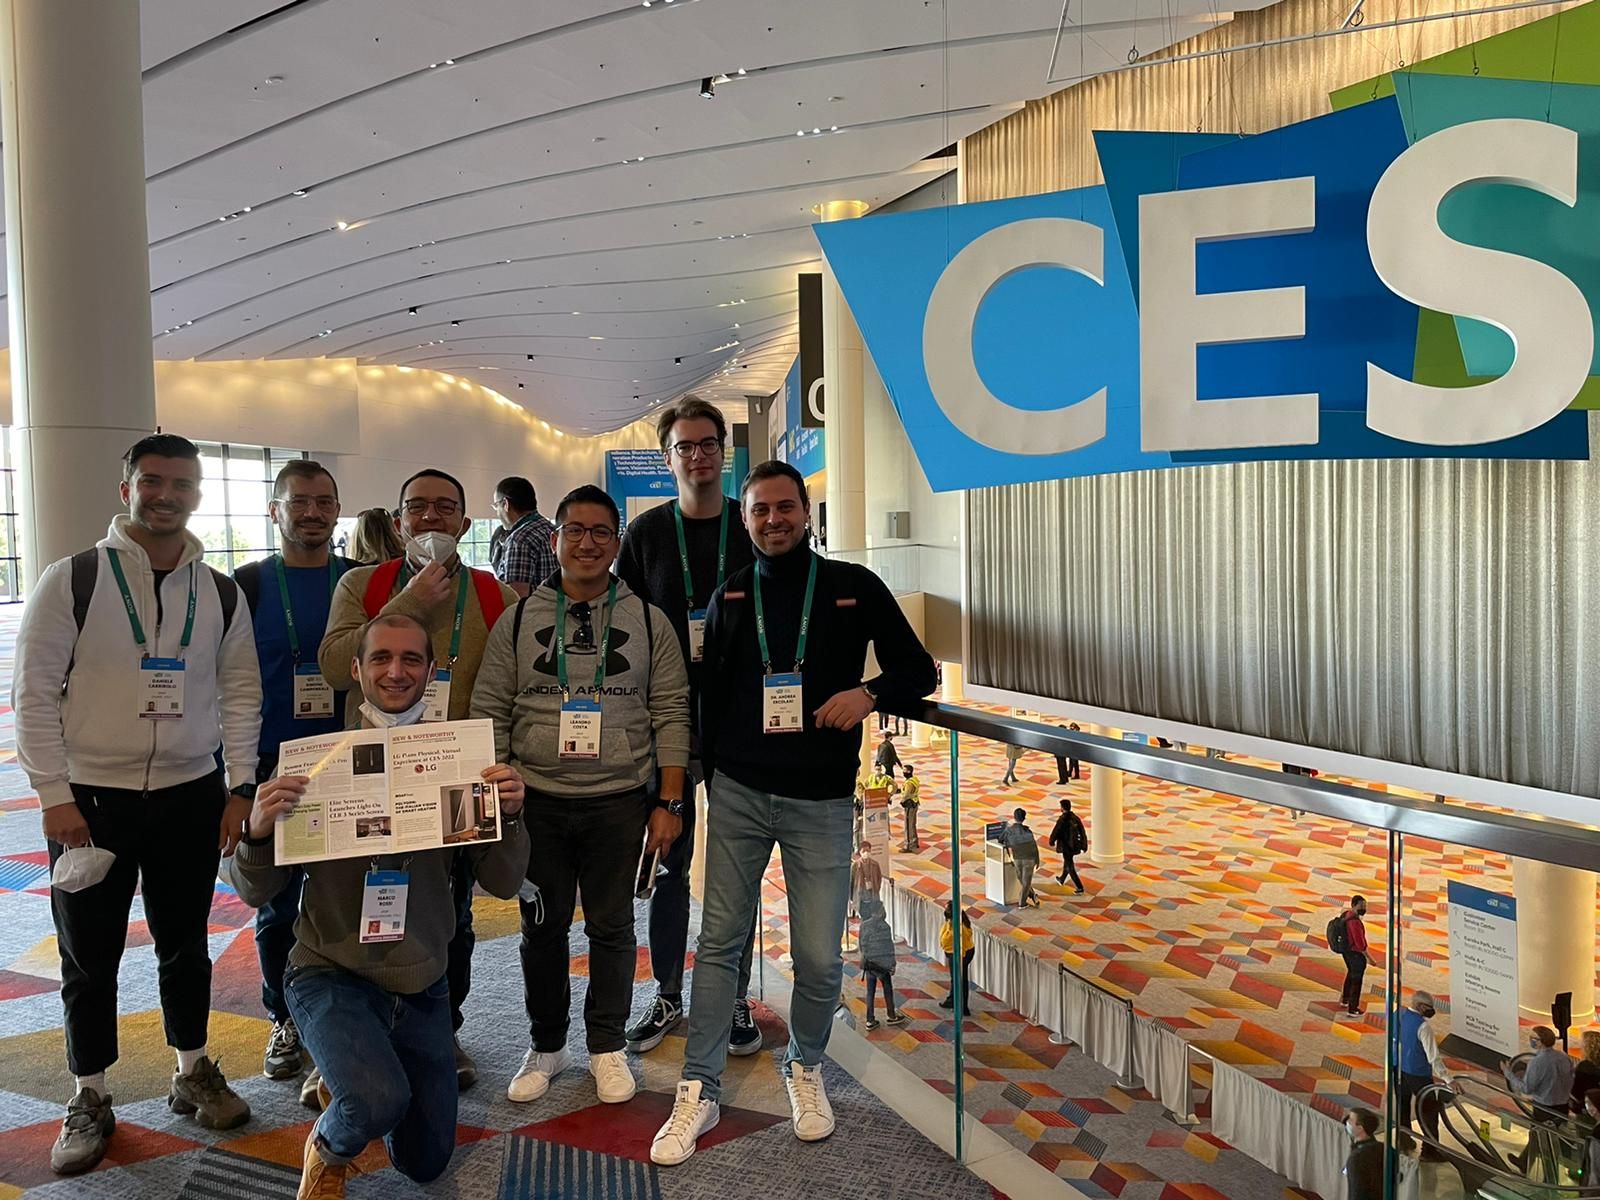
\includegraphics[width=12cm]{img/ces.jpeg}
    \caption{IRSAP ed IOTINGA al CES 2022}
    \label{fig:ces}
\end{figure}

\chapter{Definizione del problema}

Le conseguenze legali determinate dall'introduzione di un prodotto sul mercato 
sono a carico del produttore (colui che appone il proprio marchio sullo stesso). 

\section{Test di qualità}

Per quanto concerne le caratteristiche fisiche questi obblighi sono 
espressi in varie direttive europee (come la direttiva \acrshort{red} che si applica agli apparati 
radio, la direttiva \acrshort{emc} che riguarda le emissioni elettromagnetiche e la 
direttiva \acrshort{bt} che riguarda i dispositivi alimentati a tensione di rete) 
che dettano le linee guida generali da seguire per poter considerare il prodotto 
conforme (e poter apporvi il marchio \textbf{CE}). 

Le direttive impongono principi generali che essenzialmente richiedono che il 
prodotto sia realizzato \textit{a regola d'arte}. Il modo migliore (ma non l'unico)
che un produttore ha per dimostrare che il prodotto è conforme è quello di progettarlo 
seguendo le \textit{norme di prodotto} relative a quanto si sta realizzando. 

Tuttavia non è sufficiente questo per garantire la qualità: è necessario mettere 
in piedi una procedura atta a verificare che ogni esemplare prodotto sia conforme 
a quanto dichiarato. Questo si ottiene mediante procedure di \textit{quality testing}, 
ovvero dei test effettuati su ogni prodotto prima che questo lasci la fabbrica. 

Nel nostro caso questi test sono effettuati sia dal produttore della scheda elettronica, 
che collaudano ogni scheda sia a livello elettrico che funzionale, sia dal produttore finale,
ossia IRSAP stessa, che collauda ogni radiatore assemblato per garantire che funzioni correttamente 
e che non presenti pericoli (ad esempio viene verificato che non vi siano dispersioni elettriche). 

E per quanto concerne il software? Purtroppo attualmente non esistono direttive che 
impongono di seguire determinati standard per assicurarne la qualità. 

\section{Lo standard SIL}

La normativa più riconosciuta per quanto concerne il software in dispositivi embedded 
è la IEC 61508, che definisce lo standard \acrfull{sil}. 

Esso definisce 4 livelli, dal meno stringente (livello 1) al più restrittivo (4). Ogni 
livello presenta requisiti per quanto concerne la progettazione, lo sviluppo e la validazione 
del software realizzato, che sono riassunti nella seguente tabella:

\begin{center}
\begin{small}
\begin{longtable}{| p{0.18\textwidth} | p{0.18\textwidth} | p{0.18\textwidth} | p{0.18\textwidth} | p{0.18\textwidth} |}
    \hline
    \textbf{metrica} & \textbf{SIL 4} & \textbf{SIL 3} & \textbf{SIL 2} & \textbf{SIL 1} \\ \hline\hline
    Definizione delle specifiche e dei requisiti di progetto & Formale (descrizione strutturata e dettagliata dei comportamenti in linguaggio matematico) & Semi-Formale (descrizione strutturata e dettagliata dei comportamenti in linguaggio natural & Informale (descrizione in linguaggio naturale & Informale (descrizione in linguaggio naturale) \\ \hline
    Configuration-Management & Completa (automatica per sviluppo e produzione) & Completa (automatica per sviluppo e produzione) & Con l’ausilio di strumenti & Manuale \\ \hline
    Prototipazione & Si & Si & Opzionale & Opzionale \\ \hline
    Progettazione strutturata (uso di flow-chart, schemi relazionali o altro) & Si & Si & Preferenziale & Opzionale \\ \hline
    Verifica della progettazione & Si (da parte del team di progetto) & Si (da parte del team di progetto) & Si (da parte del team di progetto) & Si (esperti esterni) \\ \hline
    Project-Management & Si & Si & Si & Preferenziale \\ \hline
    Valutazione tecnica indipendente & Si & Preferenziale & Opzionale & Opzionale \\ \hline
    Analisi della gestione dei dati (necessaria per GDPR) & Si & Si & Si & Si \\ \hline
    Analisi Statistica (es. Unit Testing) & Si & Si & Opzionale & Opzionale \\ \hline
    Analisi Dinamica (es. Test automatici) & Si & Si & Si & Si \\ \hline
    Testing indipendente & Si (da org. esterna) & Si (da org. esterna) & Si (da Committente) & Opzionale \\ \hline
    Monitoraggio indipendente (test periodici) & Si (da org. esterna) & Si (da org. esterna) & Si (da Committente) & Opzionale \\ \hline
\end{longtable}
\end{small}
\end{center}

Nei progetti che sviluppiamo in IOTINGA utilizziamo solitamente il livello 2. 
Il limite principale dei livelli 3 e 4 è la definizione della specifica, che 
deve essere formale. I clienti solitamente forniscono le specifiche in linguaggio 
naturale, ed andarle ad esprimere in linguaggio formale o semi-formale è un'attività 
dispendiosa, che poco si adatta con il modello di sviluppo \textit{agile} che seguiamo. 

I prodotti infatti per rispondere alle esigenze del mercato, e per non rimanere indietro 
rispetto ai concorrenti, devono essere sviluppati velocemente, ed inoltre devono poter 
evolvere durante la loro vita con l'aggiunta di nuove funzionalità. 

\section{Necessità di test di un dispositivo IoT}

La caratteristica fondamentale per questi prodotti è l'affidabilità.
Infatti nessun utente installerebbe in casa propria un dispositivo che
non è in grado di svolgere la funzione per la quale è stato acquistato.

A maggior ragione i danni derivanti dal malfunzionamento di un impianto
di riscaldamento possono coinvolgere non solo cose, ad esempio tubature 
che si ghiacciano, ma anche estendersi a persone ed animali domestici.

È tassativo prestare attenzione alle problematiche che si possono verificare
in utenza, le quali non sono solo un danno per il cliente stesso ma anche
per l'azienda produttrice:

\begin{itemize}
    \item la prima impressione sul cliente è quella che conta, se il cliente si ritrova
        un prodotto che funziona male o addirittura non svolge la funzione prevista ne parlerà
        male, anche mediante recensioni negative online, e creerà un danno d'immagine all'azienda
        difficilissimo da sanare
    \item quando il problema si verifica dal cliente è complicata la diagnostica. I clienti,
        e spesso anche gli installatori stessi, non hanno competenze tecniche o il
        tempo da dedicare nel supportare il produttore nella ricerca del problema
    \item se il problema non è risolvibile mediante un aggiornamento \gls{firmware} è necessario
        effettuare un reso, che ha dei costi molto elevati per il produttore, in quanto
        durante il trasporto molto spesso il prodotto viene danneggiato e quindi deve
        essere rimpiazzato con un nuovo
\end{itemize}

È di fondamentale importanza assicurarsi di identificare il prima possibile quanti
più problemi possibili prima che il prodotto arrivi nelle mani dell'utente finale.

In tutto questo il software ricopre un ruolo sempre più da protagonista, in quanto
per garantire la connettività al cloud è necessario gestire una complessità elevata.

I prodotti della precedente generazione utilizzavano il software per una mera gestione
delle periferiche fisiche del prodotto, senza la necessità di interfacciarsi con sistemi
terzi. Al contrario i prodotti della attuale per svolgere tutte le funzioni di
integrazione cloud in maniera sicura richiedono un livello aggiuntivo di astrazione,
ovvero quello di un \Gls{rtos}.

Anche l'hardware stesso è più evoluto, infatti si passa dalle piattaforme ad 8 bit ai
microcontrollori a 32, con funzionalità sempre più assimilabili a quelle di un sistema
general purpose, quali ad esempio una gestione di programmazione concorrente, uno
stack di rete TCP/IP, ed una gestione della memoria virtual con MMU.

Un'altra differenza rispetto al passato è la possibilità di aggiornare il software dopo
che il prodotto lascia la fabbrica, mediante aggiornamenti di tipo \acrfull{ota}.
Questo si rende necessario non solo per la mera introduzione di nuove funzionalità in
un prodotto esistente, ma anche per mantenere il software al passo con l'evoluzione degli
altri sistemi a cui esso si collega, quale ad esempio modifiche nei protocolli di rete
dettate dall'arrivo di nuovi standard.

Sebbene l'aggiornamento consenta di risolvere problemi dopo che il dispositivo ha lasciato la
fabbrica esso comporta anche una criticità, in quanto vi è il rischio di introdurre altri problemi
in prodotti che fino a quel momento non li avevano, andando a creare un disservizio.

Bisogna infine tener conto che un prodotto di questo tipo segue un ciclo di vita molto lungo
rispetto ad esempio a PC o smartphone, che può tranquillamente superare i 10 anni dalla data di
immissione nel mercato, e l'utente si aspetta che in tutti questi anni possa continuare ad
utilizzarlo come il giorno in cui lo ha acquistato.

Conseguentemente diventa prioritario garantire i massimi livelli di qualità possibile
sul software rilasciato. Questo non si limita alla semplice assenza di bug, in quanto
questa è una garanzia che matematicamente è impossibile offrire, ma anche all'adottare
delle procedure procedure tali che consentano, dal momento che un bug si
presenta, di individuarlo e sistemarlo nel minor tempo possibile.

Tracciabilità e mantenibilità del codice sono quindi parole chiave, la prima garantisce che
sia sempre possibile risalire all'esatta versione del codice per il quale viene segnalato un
problema di modo da poterlo riprodurre, la seconda invece assicura che la soluzione al problema
sia implementabile nel minor tempo possibile e senza il rischio di regressioni.

Infine l'altro punto cardine è l'eseguire test metodologici prima che il \gls{firmware} venga
rilasciato al pubblico, sia tramite aggiornamento \acrshort{ota} che tramite installazione in fabbrica
su di un nuovo prodotto.

\section{Prassi attuale testing}

Allo stato attuale abbiamo 3 momenti di validazione di un rilascio:

\begin{enumerate}
    \item test durante lo sviluppo
    \item test di accettazione interna (effettuati da IOTINGA)
    \item test di accettazione del cliente finale (effettuati da IRSAP)
\end{enumerate}

\subsection{Test durante lo sviluppo}

Quando uno sviluppatore finisce di implementare una nuova funzionalità o risolve un
bug  prima di considerare l'attività conclusa ed integrare il
proprio lavoro nel ramo di sviluppo principale ed effettua i propri test.

Questi si occupano sia di verificare che quanto è stato implementato è conforme
alla specifica approvata dal cliente (nel caso di nuove funzionalità) oppure che
il bug sia stato risolto, sia che non siano stato modificato il funzionamento del sistema
nelle parti che sono state impattate dalla modifica.

Tali test sono a discrezione dello sviluppatore, che avendo modificato il codice sa
quali comportamenti sono impattati dalla modifica che ha realizzato e quindi devono essere
provati.

Questi test possono essere automatizzati facilmente mediante la creazione di unit-test,
che possono essere usati per validare sia le parti nuove che assicurarsi che non vi siano
regressioni che fanno smettere di funzionare quanto prima andava.

\subsection{Test di accettazione interna}

Questi test sono effettuati prima di ogni rilascio verso il cliente IRSAP.

Si occupano di validare che il software garantisca il funzionamento di una serie di casi d'uso
definiti critici, senza i quali il prodotto non sarebbe utilizzabile.
Solo se una versione del software passa tutti questi test può essere consegnata al cliente.

Essi si pongono dal punto di vista dell'utente finale, pertanto sono effettuati su un
hardware completo, isolato però dal resto del sistema, ovvero dalla componente cloud
e dall'applicazione mobile. Questo per evitare che ci sia il dubbio che il bug sia
nel cloud o nella app anziché nel dispositivo stesso.

Attualmente vengono effettuati seguendo un documento contenente una serie di scenari da testare.
Ognuno di questi è diviso in passi, e per ognuno dei quali viene indicato:

\begin{itemize}
    \item azione da compiere: un'operazione da effettuare sul sistema mediante l'interazione fisica
        con il dispositivo (pressione di pulsanti) oppure mediante cloud (tramite un apposito
        strumento che consente di simulare i messaggi inviati dal cloud e dalla app)
    \item risultato atteso: postcondizioni da verificare dopo aver effettuato l'azione, espresso in
        linguaggio non formale, ad esempio ``i \acrshort{led} sono rossi'' oppure ``entro 5 secondi viene inviato al cloud un messaggio''.
        Nel caso la postcondizione sia verificata è possibile procedere al passo successivo, altrimenti
        il test viene interrotto con esito negativo, e deve essere segnalato ad uno sviluppatore il problema.
\end{itemize}

Preferibilmente questa procedura viene fatta eseguire da chi non ha preso parte allo
sviluppo del sistema stesso. Questo per evitare che chi esegue la procedura, conoscendo
le logiche interne del software, possa essere portato a saltare o ignorare determinati
passaggi in quanto ``ovvi'', mentre chi non conosce il sistema è più propenso a seguire
i passaggi alla lettera e segnalare ogni singolo comportamento discordante con quanto
atteso.

\subsection{Test di accettazione del cliente finale}

Sul cliente finale ricade la responsabilità (anche a livello legale) del prodotto
che viene immesso sul mercato con il proprio nome sopra, e questo include anche
il software. Questo comporta il fatto che a sua volta deve svolgere dei test per
assicurarsi che il software sia conforme a quanto atteso, e nel caso segnalare i
problemi riscontrati in maniera tale che vengano corretti.

Questi test sono volti a testare tutte le funzionalità del prodotto in tutte le loro
possibili configurazioni, anche mediante l'ausilio di strumentazione altamente
specializzata quali camere climatiche per valutarne l'efficacia di termoregolazione.

Nel caso questi test abbiano successo l'artefatto testato passa da stato di candidato
al rilascio a produzione, e viene quindi installato in fabbrica su tutti i nuovi radiatori
prodotti, nonché viene lanciato un aggiornamento \acrshort{ota} su tutti i dispositivi già installati
presso i clienti finali.

\section{Problemi dell'approccio attuale}

L'approccio attuale, basato sul documento di test con fasi da seguire, presenta
alcune problematiche:
\begin{itemize}
    \item la procedura è ripetitiva, e questo può facilmente introdurre
        l'operatore che esegue i test a commettere errori, con dolo o meno
    \item l'esecuzione dei test porta via tempo, che altrimenti potrebbe essere dedicato
        a svolgere altre mansioni
    \item i test sono scritti in linguaggio naturale, non formale, e questo lascia spazio
        a libera interpretazione dalla persona che esegue i test
    \item il fatto che sia un costo eseguire la procedura fa sì che questa sia
        limitata nel numero di scenari che sono effettivamente testati
    \item per quanto detto al punto precedente il numero di build effettivamente testate
        è un sottoinsieme di quelle che vengono effettivamente effettuate, il che significa che
        i rilasci verso il cliente avvengono con meno frequenza, e si tende ad accorpare
        più funzionalità in maniera tale da effettuare un unico ciclo di test.
\end{itemize}

A questo si aggiunge il fatto che man mano che i prodotti vengono venduti il cliente ci
chiede sempre più test ad ogni release, in quanto un potenziale bug va ad impattare un numero
sempre maggiore di utenti (e quindi il danno potenziale per il produttore è sempre più grande).

Viene quindi da chiedersi se, vista la ripetitività e schematicità di queste operazioni,
sia possibile farle eseguire ad un computer, senza perdite di generalità rispetto all'esecuzione
manuale.

\section{Requisiti software per l'automazione}

Abbiamo quindi stabilito i seguenti requisiti per un sistema di automatizzazione dei test di
accettazione:

\begin{itemize}
    \item il sistema deve testare esattamente il binario che poi viene rilasciato agli utenti finali.
        Questo perché ogni alterazione, come potrebbe essere una ricompilazione del codice, può andare
        ad aggiungere errori e quindi invalidare i test effettuati
    \item l'ambiente di esecuzione (runtime environment) sul quale il test viene eseguito deve essere quanto
        più vicino possibile all'ambiente reale. Idealmente il test viene effettuato sullo stesso hardware,
        di modo da dipanare ogni possibile dubbio che il \gls{firmware} una volta installato sull'hardware abbia
        comportamenti differenti
    \item l'ambiente deve poter eseguire il \gls{firmware} in differenti configurazioni di hardware che esso supporta
        (attualmente supporta due tipologie di hardware, e ne verranno aggiunte altrettante due a breve)
    \item il sistema deve avere abbastanza flessibilità per poter validare almeno le funzionalità che oggi
        sono teste manualmente
    \item deve essere sufficientemente semplice andare ad aggiungere nuovi scenari e configurazioni da provare al sistema
    \item deve essere possibile integrare lo strumento all'interno del flusso di CI attualmente in
        uso in azienda, di modo che ogni release del \gls{firmware} prodotta venga testata senza necessità di
        un intervento manuale
\end{itemize}

% Vediamo ora cosa è disponibile in commercio per fare quanto descritto al capitolo precedente.

% \section{Strumenti di unit test}

% Una prima soluzione è quella di utilizzare gli strumenti di
% unit-test anche per effettuare i test di accettazione.
% È possibile infatti andare ad effettuare il mock di tutte le interfacce utilizzate dall'\acrshort{sdk}
% al fine di poter eseguire singoli test-case all'interno del binario.

% Questa soluzione presenta il vantaggio di poter testare in maniera veloce ed agevole
% ogni nuova release del \gls{firmware}, ma al contempo presenta alcuni svantaggi che la rendono
% inadatta allo scopo di approvare un nuovo \gls{firmware} per la produzione.

% Il problema principale è che viene testato il codice facendolo girare in un ambiente simulato,
% che per quanto simile all'ambiente reale non sarà mai completamente uguale. Soprattutto
% quando ci si interfaccia con periferiche complesse, come il \Gls{wifi}, è fondamentale che
% l'ambiente sul quale vengono eseguiti i test sia quanto più uguale possibile al runtime effettivo.

% In questo caso la soluzione migliore è effettuare i test facendo eseguire il \gls{firmware} direttamente
% all'hardware sul quale dovrà girare.

% \section{Strumenti commerciali di test elettronici}

% In commercio esistono vari strumenti che consentono di testare un dispositivo elettronico andando
% a comandare i vari input/output con i quali si interfaccia verso il mondo esterno.

% Uno di questi software è TestStand della National Instrument\footnote{https://www.ni.com/it-it/shop/software/products/teststand.html}.
% Questo software è infatti pensato per l'interfacciamento con apparecchiature di misura prodotte
% dalla medesima azienda, quali ad esempio oscilloscopi, multimetri da banco, generatori di frequenza, ecc.
% e consente di automatizzare le operazioni di test e misura.

% Come questo esistono altri software, principalmente proprietari e sviluppati internamente dalle singole
% aziende elettroniche, che svolgono la medesima funziona. Questi software tipicamente si interfacciano
% con la scheda hardware attraverso una fixture, composta da un letto di aghi conduttivi che vanno a
% fare contatto con dei test-point sulla scheda da testare.

% Questi sistemi possono benissimo essere utilizzati anche per testare il firwmare. Tuttavia non è
% il loro scopo primario, essendo pensati per identificare in primo luogo difetti nella produzione
% fisica delle schede. In particolare non offrono routine per testare componenti complesse come \Gls{wifi} o comunicazione con il
% cloud, ma si limitano a fare verifiche fra gli input e gli output.

% Inoltre l'hardware di questi dispositivi è molto costoso, essendo pensato per effettuare misurazioni
% precise a livello fisico, cosa che è fondamentale per identificare difetti sull'hardware, ma lo è
% meno per testare la release del firwmare (dove si assume che l'hardware sul quale viene lanciato il test
% sia correttamente funzionante).

\chapter{Approccio}

Prima di descrivere l'implementazione è necessario fare un passo indietro ed andare
ad analizzare con più attenzione il dispositivo \Gls{re} preso in esame.

\section{Caratteristiche hardware}

Il corpo principale dei radiatori elettrici di IRSAP è del tutto identico al radiatore idraulico,
con la differenza che il calore non viene fornito dall'acqua che circola nell'impianto ma da una 
resistenza elettrica, installata all'interno del radiatore. Il tutto viene riempito con del glicole,
per garantire una protezione antigelo, e viene sigillato con dei tappi al posto dei rubinetti di 
attacco per la mandata/ritorno dell'acqua calda.  

\subsection{Scheda elettronica}

Attualmente la gamma di radiatori elettrici IRSAP elettrificati smart include 17 prodotti distinti, 
ma ogni anno ne vengono aggiunti di nuovi. Per tutti questi progetti è quindi fondamentale, per 
questioni di ottimizzazione dei costi, avere un'elettronica quanto più possibile simile. 

Attualmente vi sono due tipologie di scheda logica che viene installata all'interno dei prodotti:

\begin{itemize}
    \item \textit{luxury}: è la versione più basilare, che viene utilizzata sulla linea di
        radiatori da bagno (chiamati anche ``scaldasalviette''). Essendo installata in ambiente 
        particolarmente umido e con il rischio di schizzi d'acqua deve sopportare un grado IP (
        misura standard del grado di protezione per componenti elettrici) superiore all'altro modello
    \item \textit{design}: è la versione riservata ai prodotti design. È la più completa,
        che offre anche modularità essendo che tutte le periferiche (pulsantiera, sensore di temperatura,
        sensore VOC, \acrshort{led}) sono collegati alla stessa con dei cavi, il che consente di inglobare l'elettronica 
        all'interno della carcassa in maniera da renderla invisibile, cosa molto importante per non rovinare 
        il desing del prodotto. Offre inoltre funzionalità aggiuntive, quali un sensore di qualità
        dell'aria (in grado di rilevare i valori di VOC e CO\textsubscript{2}) e la possibilità di
        controllare una striscia \acrshort{led} \Gls{rgbw}, utilizzata su alcuni modelli per un'illuminazione ambientale.
\end{itemize}


Ogni scheda elettronica, sia essa di tipo \textit{luxury} che \textit{design} (in \autoref{fig:schedadesign}), include le seguenti 
periferiche hardware:

\begin{itemize}
    \item un modulo \Gls{wifi} Telit GS2200M
    \item circuito di alimentazione a tensione di rete (230V AC)
    \item un circuito composto da un relè combinato ad un triac dedicato al controllo della
        cartuccia, ossia l'elemento riscaldante inserito all'interno del corpo del radiatore
    \item una sonda di temperatura \Gls{ntc} usata per misurare la temperatura ambiente
    \item una pulsantiera dotata di due pulsanti capacitivi e di \acrshort{led} RGB di illuminazione
        come feedback verso l'utente
    \item un buzzer utilizzato per un feedback uditivo della pressione dei pulsanti
    \item un circuito di lettura per il segnale \textit{\Gls{filpilote}} (il cavo nero collegato 
        in basso a destra nella scheda in \autoref{fig:schedadesign})
\end{itemize}

Oltre a quanto descritto precedentemente la versione \textit{design} include inoltre:
\begin{itemize}
    \item un sensore di qualità dell'aria in grado di
        misurare i livelli VOC e CO\textsubscript{2}
    \item la circuiteria di controllo per una striscia a \acrshort{led} \acrshort{rgbw} di illuminazione ambientale
        ed il relativo alimentatore da 230V AC a 24V DC
    \item la circuiteria di controllo per una seconda sonda di temperatura \acrshort{ntc} secondaria in grado di
        misurare la temperatura del corpo riscaldante, in maniera tale da migliorare
        l'accuratezza degli algoritmi di termoregolazione (solo per alcuni modelli)
\end{itemize}

\begin{figure}
    \centering
    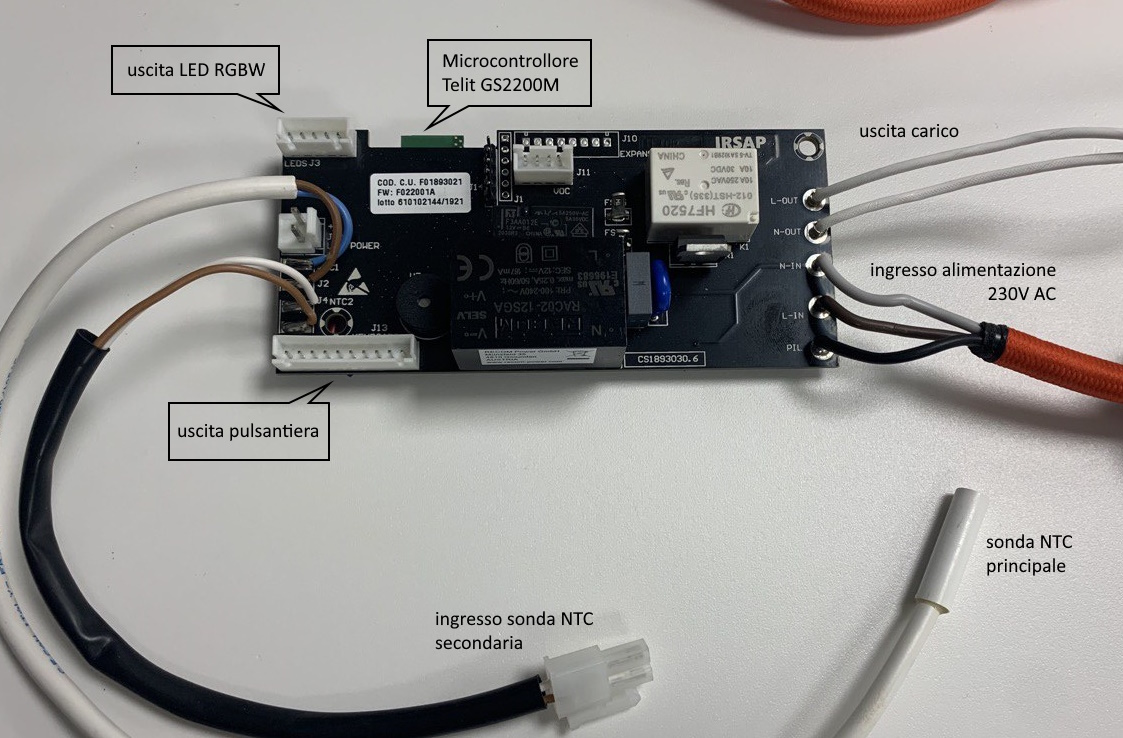
\includegraphics[width=\textwidth]{img/scheda-design.jpg}
    \caption{scheda elettronica modello \textit{design}}
    \label{fig:schedadesign}
\end{figure}
    
Entrambe le versioni di scheda elettronica eseguono la stessa versione del \gls{firmware},
che ha una fase iniziale in cui identifica la tipologia di scheda e le funzionalità
opzionali abilitate leggendole da un file di configurazione caricato nel dispositivo
in fase di collaudo, e di conseguenza configura le periferiche del \gls{micro}.

Tuttavia per essere esaustivi è necessario svolgere i test di accettazione su entrambe
le versioni di scheda elettronica, in quanto possono esservi comportamenti differenti.

\subsection{Modulo Telit}

Come cuore del sistema abbiamo il GS2200M. Questo \gls{micro} inizialmente
prodotto da Gainspan, successivamente acquisita da Telit, presenta le seguenti
caratteristiche hardware:

\begin{itemize}
    \item processore dual core \Gls{arm} Cortex M3 fino a 120Mhz, di cui un core dedicato
        alla gestione del \Gls{wifi} ed uno all'esecuzione dell'applicativo
    \item 1Mb di RAM in totale, di cui all'incirca 500kB utilizzabile dall'applicazione,
        il resto dedicata all'uso della parte \Gls{wifi}
    \item 4Mb di memoria flash interna, in parte dedicata al codice del \gls{firmware} ed
        in parte come filesystem interno in cui memorizzare i dati dell'applicazione
    \item interfaccia \Gls{wifi} b/g/n a 2.4Ghz in grado di operare sia in modalità \Gls{sta} 
        sia che \Gls{ap} a cui connettersi direttamente
    \item 19 ingressi/uscite digitali \acrfull{gpio} 
    \item 3 output \acrfull{pwm}
    \item 2 ingressi analogici mediante \acrfull{adc}, uno a 10 ed uno a 12 bit
    \item un interfaccia \Gls{i2c} hardware
    \item un interfaccia \acrfull{spi} hardware
    \item due interfacce seriali \acrshort{uart}
    \item modulo \acrfull{rtc} interno
\end{itemize}

Il microcontrollore è dotato due due core \Gls{arm}, di cui uno è deputato alla gestione
della parte \Gls{wifi} ed esegue un \gls{firmware} scritto dal produttore stesso. I due microcontrollori
comunicano attraverso una memoria condivisa (dual-port) da 64Mb. Il core principale
si occupa invece di gestire la parte applicativa.

La toolchain fornita dal produttore per lo sviluppo del \gls{firmware} in grado di girare
sul core applicativo si basa sull'ambiente di sviluppo proprietario IAR.

Viene fornito un \acrfull{sdk} che offre:

\begin{itemize}
    \item un \Gls{rtos} basato su ThreadX
    \item uno stack di rete TCP/IP basato su NetX
    \item implementazione software \Gls{wifi} sia in modalità \acrfull{sta} che \acrfull{ap},
        con relativi protocolli WEP, WPA/WPA2 sia personal che enterprise
    \item un filesystem (simile al FAT32) per la gestione della memoria flash integrata
    \item implementazione \gls{tls}
    \item implementazione client e server del protocollo \acrshort{http} ed HTTPS
    \item implementazione client del protocollo SNTP
    \item aggiornamento \acrshort{ota} con doppia partizione
    \item hardware abstraction layer (HAL) per la gestione di tutti i \Gls{gpio},
        lettura dei due \Gls{adc}, del modulo PWM, gestione del RTC, del bus i2c ed SPI
\end{itemize}

I moduli \Gls{wifi} di questo tipo possono essere utilizzati secondo due modalità:
\begin{itemize}
    \item \textit{hosted}: il modulo \Gls{wifi} viene interfacciato ad un microcontrollore
        principale che implementa le funzioni del dispositivo. Quest'ultimo si interfaccia
        con il Telit mediante interfaccia seriale e comunica con i comandi AT (standard
        per la gestione dei modem)
    \item \textit{hostless}: il modulo \Gls{wifi} esegue direttamente l'applicativo senza
        che vi sia un microcontrollore principale. Tutte le funzionalità del dispositivo
        sono implementare sul modulo Telit
\end{itemize}

Tipicamente viene seguito il primo approccio, tuttavia noi abbiamo optato per il secondo.
Questo comporta svariate semplificazioni, quali il non dover gestire la distribuzione
e l'aggiornamento di due \gls{firmware}, e l'avere quindi un prodotto più solido.

Un secondo microcontrollore comporta inoltre problemi di approvvigionamento, soprattutto di
questi ultimi periodi in cui il mercato dei componenti elettronici è impazzito, con
articoli che un tempo costavano pochi dollari arrivati a costare svariate decine.

La scelta di seguire l'approccio \textit{hostless} non è stata senza difficoltà, dovute
principalmente alla scarsa documentazione fornita dal produttore Telit. Infatti il
produttore ha deciso di seguire un approccio completamente closed-source, dove tutta
la documentazione ed il codice di esempio non è pubblico ma dato solo sotto NDA.

Questo comporta che l'unico modo per risolvere i problemi sia quello di rivolgersi
al supporto ufficiale, non trovando nulla riguardo questa particolare piattaforma
hardware con una semplice ricerca su Google. Questo ha indubbiamente reso molto più
difficoltoso lo sviluppo.

\section{Caratteristiche software}

Il \gls{firmware} è suddiviso in moduli (\textit{task}):

\begin{itemize}
    \item \textit{core}, si occupa della gestione della macchina a stati principale
        del dispositivo e del coordinamento di tutti gli altri task. Inizializza tutte
        le periferiche hardware e la rete, oltre che gestire
        gli eventi notevoli che arrivano dagli altri task
    \item \textit{termostato}, task che si occupa di tutto quel che è necessario
        per regolare la temperatura ambiente secondo le modalità di funzionamento del dispositivo,
        della lettura delle sonde ambiente/VOC, non che della gestione dell'illuminazione \acrshort{led}
        nel caso sia presente
    \item \textit{\Gls{mqtt}}, si occupa di mantenere la connessione \Gls{mqtt} verso \Gls{mqtt} IoT Core,
        sincronizzato lo stato interno del dispositivo con il server \Gls{now} mediante protocollo \Gls{mqtt}
    \item \textit{hmi}, si occupa di rispondere agli input dell'utente
        sulla pulsantiera e di darne relativo feedback mediante l'uso dei \acrshort{led} RGB e del buzzer
    \item \textit{\acrshort{http}}, si occupa di fornire mediante webserver \acrshort{http} un'API REST con
        la quale è possibile interagire direttamente con il dispositivo. È utilizzata
        per la fase di provisioning.
    \item \textit{NCM}, si occupa di gestire la connessione di rete \Gls{wifi}. Questo task
        è fornito dal produttore.
\end{itemize}

\subsection{Stati interni del dispositivo}

Il dispositivo ad alto livello può trovarsi in 3 stati distinti:

\begin{itemize}
    \item \textit{non abbinato}: in attesa di un primo abbinamento da app. Ogni funzione del
        dispositivo è esclusa finché l'utente non lo collega mediante l'applicazione
    \item \textit{disconnesso}: il dispositivo è stato in passato abbinato ma al momento non è
        connesso al cloud, perché ad esempio la connessione \Gls{wifi} non è momentaneamente disponibile
    \item \textit{connesso}: il dispositivo è connesso e sincronizzato con il cloud
\end{itemize}

\begin{figure}[ht]
    \centering
    \begin{tikzpicture}
        \node[state] (unbounded) {Non abbinato};
        \node[state, below left of=unbounded, below=1cm] (offline) {Disconnesso};
        \node[state, right of=offline] (online) {Connesso};
        \draw (unbounded) edge[bend left, align=left, right] node{abbinato\\con successo} (online)
        (offline) edge[bend left, above] node{connessione} (online)
        (offline) edge[bend left, left, align=right] node{ripristino\\di fabbrica} (unbounded)
        (online) edge[bend left, below] node{disconnessione} (offline)
        (online) edge[bend left, align=right, right] node{ripristino\\di fabbrica} (unbounded);
    \end{tikzpicture}
    \caption{Stati del radiatore}
    \label{fig:stati}
\end{figure}

Ad ogni stato del dispositivo corrisponde l'attivazione/disattivazione di uno o più
componenti software del dispositivo:

\begin{center}
\begin{tabular}{| c | c | l |}
    \hline
    stato & modo \Gls{wifi} & moduli attivi \\
    \hline
    \textit{non abbinato} & \acrshort{ap} & \acrshort{hmi}, \acrshort{http} \\
    \hline
    \textit{disconnesso} & \acrshort{sta} & \acrshort{hmi}, termostato \\
    \hline
    \textit{connesso} & \acrshort{sta} & \acrshort{hmi}, termostato, \acrshort{mqtt} \\
    \hline
\end{tabular}
\end{center}

\subsection{Termoregolazione}

La componente di termoregolazione si occupa di regolare la temperatura ambiente portandola
il più vicino possibile a quanto desiderato dall'utente (set-point) mediante
il controllo dell'accensione (on/off) dell'elemento riscaldante. Il feedback sulla
temperatura ambiente è ottenuto mediante la sonda di temperatura \acrshort{ntc}.

Il dispositivo ha diversi modi di funzionamento:
\begin{itemize}
    \item \textit{standby}: dispositivo completamente spento, sia per quanto riguarda il riscaldamento
        che per l'illuminazione \acrshort{led}
    \item \textit{antigelo}: il dispositivo mantiene una temperatura di sicurezza (impostata dall'utente)
        per prevenire danni dati da una temperatura ambiente troppo bassa (ad es. congelamento delle tubature)
    \item \textit{vacanza}: all'interno di un intervallo temporale impostato dall'utente funziona
        in modalità antigelo
    \item \textit{away}: imposta un set-point ridotto (ECO) in quanto l'utente non è in casa
    \item \textit{programmato}: segue una programmazione settimanale che consente per ogni
        giorno della settimana di creare fino ad 8 fasce orarie
    \item \textit{manuale temporaneo}: segue un set-point manuale per un determinato tempo
    \item \textit{manuale}: segue il set-point utente che è fisso e non varia mai
        configurato dall'utente, quindi torna a funzionare nella modalità precedente
    \item \textit{\gls{filpilote}}: il dispositivo è controllato (ove disponibile) da un segnale
        esterno in ingresso sul cavo \Gls{filpilote}
\end{itemize}

È possibile mediante interfaccia utente muoversi fra le varie modalità come dettagliato
in \autoref{fig:modi}.

\begin{figure}[ht]
    \centering
    \begin{tikzpicture}
        \node[state] (programmato) {Programmato};
        \node[state, right of=programmato, align=center] (manuale-tempo) {Manuale\\temporaneo};
        \node[state, right of=manuale-tempo] (manuale) {Manuale};
        \draw (manuale) edge[loop above] node{modifica set-point} (manuale)
            (programmato) edge[bend left, above] node{modifica set-point} (manuale-tempo)
            (manuale-tempo) edge[bend left, above] node{modifica set-point} (manuale);
    \end{tikzpicture}
    \caption{Modi del radiatore}
    \label{fig:modi}
\end{figure}

\subsection{Comunicazione cloud}

La componente cloud è implementata su \Gls{mqtt}. La connessione avviene grazie al protocollo
\Gls{mqtt} usando il servizio broker di \Gls{mqtt}, IoT Core.

\subsubsection{Autenticazione}
La connessione è cifrata mediante \gls{tls} 1.2 ed autenticata mediante certificato del client.

Tale certificato è generato per ogni singolo dispositivo durante le fasi di produzione,
e viene firmato da una \acrfull{ca} intermedia del produttore hardware, come nel seguente schema:

\begin{figure}[ht]
    \centering
    \begin{tikzpicture}
        \node[rectangle, draw, align=center, inner sep=8pt] (root) {root \acrshort{ca} \\ \Gls{mqtt}};
        \node[rectangle, draw, right of=root, align=center, inner sep=8pt] (intermedia) { \acrshort{ca} intermedia\\ produttore};
        \node[rectangle, draw, right of=intermedia, align=center, inner sep=8pt] (dispositivo) {certificato \gls{tls}\\ dispositivo};
        \draw (root) edge[above] node{firma} (intermedia)
            (intermedia) edge[above] node{firma} (dispositivo);
    \end{tikzpicture}
    \caption{Catena \gls{tls}}
    \label{fig:tls-chain}
\end{figure}

La \acrshort{ca} intermedia è generata e firmata dalla  \acrshort{ca} generale di \Gls{mqtt} \Gls{iotcore}. In questo
modo è possibile generare in fase di programmazione offline un certificato per ogni
dispositivo che deve essere prodotto. Alla prima connessione del dispositivo al \gls{cloud} questo
automaticamente si registrerà all'interno di \Gls{iotcore} senza ulteriori necessità di interventi manuali.

\Gls{iotcore} permette di associare ad ogni certificato una policy, che può andare a garantire al
client dei permessi per quanto riguarda \Gls{mqtt}:
\begin{itemize}
    \item \textit{connect}: autorizza il client a connettersi ad \Gls{iotcore} utilizzando un particolare
        \textit{clientId}
    \item \textit{publish}: consente al cilent di pubblicare su determinati \gls{topic} \Gls{mqtt}
    \item \textit{subscribe}: consente al dispositivo di effettuare una subscription su determinati \gls{topic}
        al fine di ricevere aggiornamenti in tempo reale dal \gls{cloud}
\end{itemize}

La policy predefinita restringe i permessi ai soli \gls{topic} dedicati per il client con il determinato certificato
che si connette al cloud. Per fare questo all'interno del \gls{topic} viene inserito il seriale dello specifico
dispositivo, che è lo stesso contenuto all'interno del certificato.

\subsubsection{Protocollo stateless di comunicazione}

Per quanto concerne il protocollo di comunicazione in origine abbiamo valutato inizialmente
l'uso del protocollo Device Shadowing\footnote{\url{https://docs.aws.amazon.com/it\_it/iot/latest/developerguide/iot-device-shadows.html}}
supportato nativamente da \Gls{mqtt} \Gls{iotcore}.

Tuttavia, tale protocollo aveva delle limitazioni che non ne consentivano l'utilizzo nella nostra
applicazione, in particolare:

\begin{itemize}
    \item il pacchetto viene codificato in \acrshort{json}, il che presenta un overhead di memoria
        e CPU notevole per il microcontrollore scelto. Inoltre la codifica \acrshort{json} può
        introdurre dei bug di encoding
    \item vi è un hard-limit di 8Kb di dimensione massima di un documento di stato (shadow).
        Questo, seppur poteva essere sufficiente nelle prime versioni del prodotto, andava
        a limitare possibilità di espansione futura del prodotto
    \item il protocollo di comunicazione trasferisce dei delta, che sebbene riducano la
        dimensione di un pacchetto di dati rendono più complessa la sincronizzazione degli
        stati del sistema
\end{itemize}

Per tutte queste ragioni abbiamo scelto di adottare un protocollo binario proprietario,
tramite il quale andiamo a trasferire stati completi del dispositivo.

Abbiamo deciso di mantenere comunque i concetti di alto livello dati dal protocollo \Gls{mqtt}
Device Shadowing, in particolare la nomenclatura \textit{shadow} per indicare uno stato del
dispositivo, che è suddiviso in:
\begin{itemize}
    \item \textit{state desired} come lo stato in cui si vuole portare il dispositivo, ovvero le
        impostazioni che l'utente può modificare agendo dalla app, quali ad esempio la modalità di funzionamento,
        la programmazione oraria, la configurazione dei \acrshort{led} RGB, etc.
    \item \textit{state reported} lo stato attuale del dispositivo. È un superset dello stato
        desired, in quanto oltre a tutti i campi di quest'ultimo include anche tutti quei valori
        in sola lettura (ovvero che solo il dispositivo può modificare), ovvero i parametri
        statistici e di monitoraggio quali la temperatura ambiente, il livello di qualità dell'aria (VOC),
        gli allarmi del dispositivo, la qualità della connessione \Gls{wifi}, etc.
\end{itemize}

Il protocollo è quindi stateless, e consente di effettuare 4 messaggi, più relative risposte,
(come visibile in \autoref{fig:comunicazione_cloud}):

\begin{itemize}
    \item \textit{get}: disponibile fra dispositivo e cloud, consente la richiesta dello stato \textit{desired} corrente
    \item \textit{reported-update}: disponibile fra dispositivo e cloud, trasmette lo stato
        completo del dispositivo al server
    \item \textit{delete}: eliminazione dello stato corrente presente su cloud
    \item \textit{desired-update}: unico messaggio inviato dal cloud al dispositivo,
        trasmette lo stato completo desired
\end{itemize}

Il tipo di messaggio dipende dal \gls{topic} \Gls{mqtt} sul quale i pacchetti sono pubblicati. Ad
un messaggio pubblicato dal dispositivo verso il server il server risponde in base allo
stato della richiesta sullo stesso \gls{topic} con aggiunto un suffisso:
\begin{itemize}
    \item \texttt{/accepted}: la richiesta è stata accettata dal server
    \item \texttt{/rejected}: la richiesta è stata respinta dal server in quanto è
        avvenuto un errore
\end{itemize}

\begin{figure}[ht]
    \centering
    \begin{tikzpicture}
        \node[rectangle, minimum height=1cm, draw] (dispositivo) {\Gls{re}};
        \node[rectangle, minimum height=1cm, draw, right of=dispositivo] (cloud) {Cloud \Gls{mqtt}};
        \draw (dispositivo) edge[bend left=40, above] node{\textit{get}} (cloud)
            (dispositivo) edge[bend left=10, above] node{\textit{reported-update}} (cloud)
            (dispositivo) edge[bend right=10, below] node{\textit{delete}} (cloud)
            (cloud) edge[bend left=40, below] node{\textit{desired-update}} (dispositivo);
    \end{tikzpicture}
    \caption{Schema di comunicazione dispositivo/cloud}
    \label{fig:comunicazione_cloud}
\end{figure}

Il client può identificare a quale richiesta fa riferimento ad una risposta attraverso un
token (\textit{clientToken}) che il client setta su ogni richiesta inviata e che il server aggiunge
ad ogni risposta che invia al client.

\subsubsection{Formato messaggi cloud}

Ogni messaggio su cloud include un header fisso, che comprende i seguenti campi

\begin{center}
\begin{longtable}{| p{5cm} | c | p{8cm} |}
    \hline
    \textbf{chiave} & \textbf{tipo} & \textbf{descrizione} \\ \hline
    timestamp & u32 & timestamp di invio del messaggio \\ \hline
    clientToken & u32 & un ID della richiesta che il client aggiunge ad ogni messaggio
        per poter correlare le risposte alle richieste effettuate \\ \hline
    version & u32 & versione del messaggio \\\hline
    length & u16 & lunghezza totale del messaggio (header incluso) \\ \hline
    type & u8 & tipo di messaggio, identifica il payload presente \\ \hline
\end{longtable}
\end{center}

A seguire nel messaggio è presente il payload:

\begin{center}
\begin{longtable}{| p{5cm} | c | p{8cm} |}
    \hline
    \textbf{chiave} & \textbf{tipo} & \textbf{descrizione} \\ \hline
    connected & u8 & 1 se il dispositivo è online, altrimenti 0 \\ \hline
    firmwareVersion & u8[2] & versione \gls{firmware} (major, minor) \\ \hline
    hardwareVersion & u8 & versione hardware \\ \hline
    macAddress & u8[6] & MAC address (seriale del dispositivo) \\ \hline
    systemStatus & u8 & stato del Sistema (bitmask) \\ \hline
    filPiloteStatus & u8 & stato ingress Fil Pilote \\ \hline
    alarm & u8 & allarmi (bitmask)\\ \hline
    heatingStatus & u8 & stato riscaldamento (bitmask)\\ \hline
    RSSI & u8 &Potenza \Gls{wifi}\\ \hline
    noise & u8 &Rumore \Gls{wifi}\\ \hline
    currentSetPoint & i16 & set point corrente (in decimi di grado)\\ \hline
    currentSetPointEnd & u32 & scadenza set-point corrente\\ \hline
    vocValue & u16 & valore VOC (qualità dell’aria)\\ \hline
    co2Value & u16 & valore CO2 (qualità dell’aria)\\ \hline
    temperature & i16 & temperature ambiente (in decimi di grado)\\ \hline
    setPointOff & u16 & set point di OFF (espresso in decimi di grado)\\ \hline
    setPointEco & u8 & set point di ECO (espresso in decimi di grado - 10C)\\ \hline
    manualSetPoint & u8 & set point manual (espresso in decimi di grado -10C)\\ \hline
    temporaryManualSetPoint & u8 & set point manual temporaneo (in decimi di grado)\\ \hline
    temporaryManualEnd & u32 & fine manuale temporaneo (timestamp)\\ \hline
    hysteresis & u8 & isteresi (espressa in decimi di grado)\\ \hline
    temperatureSensorOffset & i8 & correzione sensore di temperature (espresso in decimi di grado)\\ \hline
    loadTemperature & i16 & temperature carico (in decimi di grado)\\ \hline
    loadOnSeconds & u32 & cumulativo in secondi di accensione del carico\\ \hline
    holidayStart & u32 & timestamp inizio vacanza\\ \hline
    holidayEnd & u32 & timestamp fine vacanza\\ \hline
    metricInterval & u8 & intervallo invio metriche periodiche (minuti)\\ \hline
    systemId & u8[16] & ID impianto (UUID)\\ \hline
    timezone & i16 & offset timezone rispetto ad orario UTC\\ \hline
    systemConfiguration & u8 & configurazione di sistema (bitmask)\\ \hline
    ipAddress & u8[4] & indirizzo IP \Gls{wifi}\\ \hline
    openWindowOffTime & u8 & tempo di spegnimento in caso rilevamento finestra aperta\\ \hline
    ledManualSetPoint & u32 & colore \acrshort{led} ambiente (HSV)\\ \hline
    schedule & u8[196] & programmazione riscaldamento\\ \hline
    ledSchedule & u8[196] & programmazione \acrshort{led} (stesso formato di prima)\\ \hline
    ledEnabled & u8 & \acrshort{led} ambiente on/off\\ \hline
    ledMode & u8 & modalità led ambiente (manuale/programmato)\\ \hline
    ledColor & u32[10] & preset colori \acrshort{led} ambiente per uso in fasce orarie\\ \hline
    temporaryManLedSP & u32 & set point \acrshort{led} manuale a tempo\\ \hline
    temporaryManLedSPEnd & u32 & fine manuale a tempo \acrshort{led}\\ \hline
    estimatedTemperature & i16 &temperatura ambiente (scritta da cloud per uso con altri sensori)\\ \hline
    externalTemperature & i16 & umidità esterna (scritta da cloud)\\ \hline
    estimatedHumidity & u8 & umidità ambiente (scritta da cloud)\\ \hline
    externalHumidity & u8 & umidità esterna (scritta da cloud)\\ \hline
    currentLedSetPoint & u32 & set point \acrshort{led} corrente\\ \hline
    currentLedSetPointEnd & u32 & fine fascia oraria \acrshort{led} corrente\\ \hline
    cartridgePowerWatts & u16 & potenza della cartuccia\\ \hline
    totConsumption & u32 & consumo cumulato in tutta la vita del radiatore\\ \hline
    totConsumptionValue & u32 & valore all’ultimo snapshot di consumo\\ \hline
    totConsumptionTime & u32 & consumo all’ultimo snapshot\\ \hline
    modelName & char[32] & nome modello del radiatore\\ \hline
\end{longtable}
\end{center}

\subsection{API di configurazione locale}

Quando il dispositivo viene acceso per la prima volta è necessario fornirgli la
configurazione della rete \Gls{wifi} e l'identificativo (UUID) dell'impianto al quale
collegarsi prima che esso possa iniziare a funzionare.

Per fare ciò il dispositivo mette a disposizione un'API REST attraverso la quale la
app \Gls{now} comunica attraverso una connessione \Gls{wifi} diretta (in questa fase
il dispositivo imposta la propria interfaccia \Gls{wifi} in modo \acrshort{ap}).

Mette a disposizione le seguenti API REST:

\begin{center}
\begin{tabular}{| l | c | p{6cm} |}
    \hline 
    \textbf{endpoint} & \textbf{metodo} & \textbf{descrizione} \\ \hline 
    \texttt{/irsap/state} & GET & ottiene lo stato corrente del dispositivo \\ \hline 
    \texttt{/irsap/wifi/scan} & GET & ottiene l'elenco di reti \Gls{wifi} visibili dal dispositivo \\ \hline 
    \texttt{/irsap/provision} & POST & invia al dispositivo la configurazione \\ \hline 
    \texttt{/irsap/test} & POST & attiva la modalità collaudo del dispositivo \\ \hline 
    \texttt{/gainspan/system/fwup} & POST & invia un aggiornamento \gls{firmware} al dispositivo \\ \hline
\end{tabular}
\end{center}

\subsection{HMI}

L'interfaccia utente del dispositivo si compone di due pulsanti, \textbf{+} e \textbf{-},
i \acrshort{led} RGB di illuminazione della pulsantiera ed il buzzer.

Tramite l'\acrshort{hmi} è possibile effettuare le seguenti operazioni:

\begin{itemize}
    \item pressione breve \textbf{+}: incrementa il set-point corrente
    \item pressione breve \textbf{-}: decrementa set-point corrente
    \item pressione per più di 3 secondi (ma meno di 5) del tasto \textbf{-}:
        attiva modalità \textit{antigelo}
    \item pressione per più di 5 secondi del tasto \textbf{-}: attivazione modalità
        \textit{stand-by}
    \item pressione prolungata dei tasti \textbf{+} e \textbf{-} per più di 5 secondi:
        ripristino impostazioni di fabbrica
\end{itemize}

I \acrshort{led} invece sono utilizzati per segnalare la temperatura impostata dall'utente
(in base al set-point passano da un colore più freddo ad uno più caldo), sia ad
indicare condizioni particolari quali radiatore non abbinato (\acrshort{led} rossi), connessione
in corso (viola lampeggiante), modo \textit{stand-by} (viola fisso) o \textit{antigelo} (bianco).

\section{Interfacciamento con il sistema di test}

Ora che abbiamo visto a grande linee come è strutturato il dispositivo sia dal punto
di vista hardware che software, possiamo affermare che il software presente al suo interno
può interagire con il mondo esterno essenzialmente in tre modi:

\begin{enumerate}
    \item comunicazione cloud: invio e ricezione di stati completi (\textit{shadow})
        mediante il collegamento \Gls{mqtt} al cloud \Gls{iotcore}
    \item comunicazione locale: invio e ricezione di comandi mediante l'API REST locale
    \item fenomeni fisici: calore emesso, pulsanti che vengono premuti, luce e suoni
        emessi, temperatura ambiente che varia
\end{enumerate}

Riguardo ai primi due punti è facile pensare ad un sistema per automatizzare e programmare
le interazioni, passando da interfacce digitali. Il problema è quindi l'interazione fisica
con il dispositivo, che passa per fenomeni analogici.

Possiamo pensare a tre modi:

\begin{itemize}
    \item interazione con il dispositivo fisico
    \item interazione con la scheda elettronica
    \item esecuzione del \gls{firmware} in un emulatore
\end{itemize}

\subsection{Interazione con il dispositivo fisico}

Una prima possibilità che si pensa potrebbe essere quella di piazzare il radiatore in una camera
climatica e mediante sensori ed attuatori interagire sul dispositivo stesso come farebbe
un essere umano.

Questo garantisce di testare uno scenario del tutto identico a quel a cui sarebbe
difronte l'utente che si installa il termosifone in casa, tuttavia presenta alcune
problematiche che rendono questa strada non percorribile.

Prima di tutto necessita di strumentazione molto specifica e costosa (le camere climatiche),
che sebbene a disposizione di IRSAP sono occupate per altri scopi, come lo sviluppo e
la validazione degli algoritmi di termoregolazione.

In secondo luogo i test dovrebbero necessariamente seguire le tempistiche dettate dai processi
fisici che vengono governati, come il riscaldamento di una stanza.
Questo rende il test molto lungo in termini temporali, anche svariate ore per eseguire ogni singolo
passaggio, considerando che l'ambiente andrebbe ripristinato a pari condizioni iniziali prima
di poterne eseguire uno nuovo.

\subsection{Interazione con la sola elettronica}

Viene da pensare che si possa quindi eliminare il resto del sistema (il radiatore
stesso) e concentrarsi quindi sul test della sola scheda elettronica, andando a
simulare gli ingressi e le uscite con cui la scheda comunica con le periferiche
a cui è solitamente collegata. Questa è una possibilità che viene effettivamente
utilizzata in fase di collaudo dell'elettronica, quando è necessario assicurarsi ad
esempio che non vi siano stati problemi di produzione quali saldature fredde.

Tuttavia presenta una problematica la scheda del radiatore è alimentata con
la tensione di rete a 230V, il che rende necessario dover isolare la scheda rispetto
al dispositivo con cui la si interfaccia per ragioni sia di sicurezza elettrica sia
di possibili danni che possono essere arrecati al dispositivo che lavora a bassa tensione.

In effetti possiamo pensare che non ci serva interfacciare la scheda elettronica
vera e propria del radiatore: dopotutto a noi interessa testare la componente software,
che gira sul microcontrollore presente sulla scheda, assumendo che l'elettronica è
funzionante come da specifica (in quanto già collaudata in fase di produzione).

Possiamo quindi isolare solo la parte che ci interessa, ovvero il chip Telit, utilizzando
un kit di sviluppo fornito direttamente dal produttore. Questo permette di connettere
la nostra interfaccia di test con tutti gli input/output digitali (\Gls{gpio}) della scheda,
così che potremo andare a simulare tutte le periferiche hardware più agevolmente via software.

Questa è la soluzione che alla fine ho scelto.

\subsection{Esecuzione del firmware in un emulatore}

Infine un'ultima possibilità è quella di eseguire il \gls{firmware} non sull'hardware
reale ma su un sistema emulato.

Questo presenta alcune problematiche, in particolare essendo la piattaforma Telit
proprietaria è difficile carpirne tutte le specifiche di funzionamento per andare
ad emularne in maniera quanto più simile possibile il funzionamento.

Si potrebbe quindi decidere di compilare un binario x86, andando a sostituire tutte
le funzioni utilizzate del framework Telit con stub implementati ex-novo. Questo
sebbene potrebbe funzionare (anche se il suo sviluppo sarebbe molto lungo e dispendioso)
avrebbe come effetto che non si sta effettivamente testando il binario che poi andrà
in produzione, compresa l'integrazione con l'\acrshort{sdk} e le caratteristiche fisiche dell'hardware.

Ho quindi deciso di escludere questa strada, che invece è percorribile su altre
piattaforme hardware quali l'ESP-32, in quanto utilizza un \acrshort{sdk} completamente open-source,
e mette già a disposizione la possibilità di emulare un hardware con il software \textit{qemu}.

\chapter{Implementazione}

In questo capitolo vediamo come il sistema di test descritto sopra è stato implementato.

\section{Interfacciamento hardware}

Come già detto in precedenza ho scelto di interfacciarmi direttamente con un kit
di sviluppo del microcontrollore scelto, come si può vedere in \autoref{fig:quadretto}.

Il kit di sviluppo mette a disposizione tutti i pin connessi al microcontrollore
su comodi pin header. Integra inoltre un convertitore \Gls{uart} (seriale) - \acrshort{usb} per
permettere di programmarlo e per interagire con la eventuale console di debug
(che il radiatore mette a disposizione).

Tutti gli I/O lavorano nel dominio dei 3.3v, quindi ho scelto di utilizzare un
Raspberry Pi come interfaccia hardware, connettendo direttamente i sui \Gls{gpio} con
quelli del kit di sviluppo.

Questo ha un'unica limitazione, che è quella che il Raspberry Pi non mette a disposizione
uscite analogiche (DAC), che sarebbero utili per simulare la lettura del sensore di
temperatura. Tuttavia con un uscita PWM ed un opportuno filtro analogico passivo è
possibile comunque simularne il valore, fosse necessario. Nel mio caso ho scelto di
non realizzare questo circuito, connettendo una resistenza fissa al sensore di
temperatura del radiatore, in quanto non rientra negli scopi di questi test la lettura
di valori differenti del sensore di temperatura (che dipende da caratteristiche fisiche
del sensore più che dal software).

Il raspberry dispone inoltre di un'interfaccia \Gls{wifi} a 2.4Ghz che consente quindi di
avere tutto quanto server per il testing del dispositivo in un'unico comodo dispositivo.

\begin{figure}
    \centering
    \includegraphics[width=\textwidth]{img/devkit.png}
    \caption{Hardware di test realizzato}
    \label{fig:quadretto}
\end{figure}

\section{Motore di esecuzione test}

Per la componente software ho deciso di utilizzare il linguaggio di programmazione
Python. Questa scelta è motivata sia dalla versatilità che offre nell'interazione anche
di basso livello con funzionalità del sistema operativo e periferiche, sia dal fatto
che è il linguaggio che solitamente viene utilizzato in azienda per la scrittura di
tools e script.

Il codice è realizzato come una libreria python, \texttt{fw\_test}, sotto forma di
un pacchetto installabile con \textit{pip}. In questa maniera l'interfacciamento
verso l'hardware e la fixture di test viene separata dal codice effettivo dei test,
che può potenzialmente risiedere anche su un repository separato.

La libreria mette a disposizione un oggetto principale \texttt{Context} che, una
volta instanziato con un suo file di configurazione, mette a disposizione una serie
di interfacce che consentono l'interazione con i vari moduli visti poc'anzi:

\begin{itemize}
    \item \texttt{io}: è responsabile a gestire tutte le periferiche di I/O
        verso la scheda, ossia \Gls{gpio} e \Gls{uart} di debug. Mette a disposizione dei metodi di
        alto livello per interagire con la scheda e verificare lo stato del dispositivo,
        quali ad esempio \texttt{get\_status\_led\_color()} che ottiene il colore del
        \acrshort{led} di stato, oppure \texttt{press\_plus()} che invia la pressione del stato \texttt{+}.
    \item \texttt{cloud}: è il modulo responsabile all'interazione con il cloud. Si
        occupa di mantenere attiva la connessione \Gls{mqtt} con il broker \Gls{mqtt} IoT Core,
        gestire la codifica/decodifica di messaggi da oggetti a binario e vice versa,
        di interfacciarsi con la gestione dei \Gls{awsjob} per la distribuzione di aggiornamenti
        \acrshort{ota}.
    \item \texttt{wifi}: è il modulo deputato al controllo dell'interfaccia \Gls{wifi}
        della raspberry. Consente di cambiare la modalità fra \acrshort{ap} e \acrshort{sta},
        supportando l'uso di configurazioni differenti di access point.
    \item \texttt{api}: implementa l'API REST di comunicazione locale con il dispositivo,
        che come detto è usata dalla app in fase di abbinamento del dispositivo
\end{itemize}


Come motore di esecuzione dei test ho deciso di utilizzare \textit{pytest}, che
è lo standard de factor in ambiente Python. Definendo un file \texttt{conftest.py}
sono andato a meglio adattare il sistema di test per integrarlo con la libreria
sviluppata sopra. In particolare il motore di test:

\begin{itemize}
    \item si occupa di instanziare la libreria \texttt{fw\_test} prima dell'avvio
        dei test, ed a terminarla una volta terminati tutti i test
    \item prima di ogni test, si preoccupa di portare il sistema in uno stato normale,
        ovvero il dispositivo deve avere in esecuzione la versione \gls{firmware} sotto test
        e deve essere resettato
    \item raccoglie i log dai vari moduli, inclusa la libreria \texttt{fw\_test} che
        usa il modulo logging standard di Python. In questo modo quando un test
        fallisce si può risalire alle operazioni che ha fatto il Raspberry per causare
        il fallimento, in modo da poter più agevolmente riprodurre il problema
\end{itemize}

\subsection{Interfacciamento con l'I/O}

Per l'interfacciamento con l'I/O ho deciso di utilizzare la libreria di riferimento
per comunicare con i \Gls{gpio} del Raspberry Pi.

In una prima fase vengono inizializzati tutti i pin in base alla loro funzione, input
o output, e viene aperta l'interfaccia seriale \Gls{uart} con la quale si può comunicare con
il kit di sviluppo.

I messaggi di debug del radiatore vengono quindi catturati e convogliati sul logger
di sistema, di modo che poi siano raccolti dal sistema CI (continuos integration)
e raccolti per scopi di debugging di eventuali test falliti.

Vengono inoltre offerti dei metodi di alto livello per interagire con le varie
periferiche del dispositivo, ad esempio ottenere il colore dei led, premere un
pulsante sulla pulsantiera, riavviare il dispositivo, etc.
Inoltre sono creati dei wrapper per i comandi seriali più comuni da mandare al
radiatore.

\subsection{Interfacciamento con il cloud}

Come visto in precedenza il dispositivo si collega al cloud \Gls{mqtt} IoT Core mediante
autenticazione con certificato client. Essendo il meccanismo di autenticazione con il
server oggetto stesso del test, ed essendo che il broker \Gls{mqtt} IoT Core non è installabile
su un normale computer essendo una componente proprietaria, è impossibile testare il
dispositivo facendolo collegare ad un \Gls{mqtt} broker differente (come può essere Mosquitto \Gls{mqtt}).

Inoltre IoT Core mette a disposizione alcune funzionalità che non sono disponibili in
altri broker. In particolare la funzionalità dei job, ossia dei processi batch che è
possibile schedulare e fare eseguire ai dispositivi, che consentono di distribuire l'esecuzione
di operazioni. Noi utilizziamo principalmente i job per la distribuzione degli aggiornamenti \acrshort{ota},
ma anche per altre operazioni di servizio (come l'aggiornamento di alcuni dati statistici).

Per questo motivo la cosa più semplice è utilizzare IoT Core stesso, ma isolare il collegamento
fra il broker ed il resto del sistema per il dispositivo sotto test. Il che si traduce nel
fatto che le regole che azionerebbero il resto del sistema ad un evento di pubblicazione
sui \gls{topic} usati dal cloud sono disabilitate per il seriale del dispositivo in test.

Il raspberry di test si interfaccia quindi con IoT Core come client \Gls{mqtt} che può
andare a pubblicare/sottoscriversi ai \gls{topic} su cui il dispositivo comunica, come vediamo in \autoref{fig:cloud}.
Dato che il broker non ha un ruolo attivo nel sistema (si occupa solo di inoltrare i messaggi ma non
applica alcuna logica di protocollo) la sua presenza all'interno dello scenario di test non
è problematica, in quanto viene trattato come un qualsiasi dispositivo di infrastruttura
(come ad esempio può essere un router su internet).

\begin{figure}[h]
    \centering
    \begin{tikzpicture}
        \node[cloud, draw,cloud puffs=10,cloud puff arc=120, aspect=2, inner ysep=1em] (cloud) {\Gls{mqtt} IoT};
        \node[below of=cloud, left of=cloud, node distance=3cm, rectangle, draw, inner sep=8pt] (dispositivo) {\Gls{re}};
        \node[below of=cloud, right of=cloud, node distance=3cm, rectangle, draw, inner sep=8pt] (raspberry) {Raspberry Pi};
        \draw (dispositivo) edge[bend left, left, align=center] node[left=0.5cm]{\Gls{mqtt}\\certificato} (cloud)
            (raspberry) edge[bend right, right, align=center] node[right=0.5cm]{\Gls{mqtt} su Websocket\\autenticazione IAM} (cloud);
    \end{tikzpicture}
    \caption{interfacciamento fra raspberry e cloud}
    \label{fig:cloud}
\end{figure}


A livello implementativo uso per collegare il software ad IoT Core
la libreria ufficiale di AWS, \textit{awsiotsdk}. Questa libreria, a differenza dei
normali client \Gls{mqtt}, consente infatti di autenticarsi grazie a credenziali IAM, non
richiedendo quindi la generazione di certificati per il tool di test.

Il modulo cloud del sistema di test, oltre a gestire a basso livello la connessione
al server \Gls{mqtt}, aggiunge un layer di astrazione che automatizza la conversione fra
binario e oggetti Python, e vice versa, dei messaggi secondo il protocollo custom
implementato.

È fornito un metodo \texttt{publish(msg)} per inviare un messaggio, che viene codificato ed
inviato sul \gls{topic} opportuno (scelto in base al tipo di messaggio secondo la specifica
del protocollo). Ad ogni messaggio ricevuto sui \gls{topic} a cui il dispositivo fa la
subscription viene decodificato e salvato in una coda. Viene fornito un metodo \texttt{receive(timeout)}
per ricevere un messaggio, ossia scodare l'ultimo messaggio dalla coda, o attendere
fino ad un dato timeout che arrivi un messaggio dal dispositivo.

Per quanto concerne la gestione degli \Gls{mqtt} IoT Core Jobs, che come detto prima vengono
utilizzati per distribuire sui dispositivi operazioni batch da eseguire, viene
utilizzata la libreria ufficiale Python di \Gls{mqtt} \textit{boto3}. Vengono fornite
3 interfacce:
\begin{itemize}
    \item \texttt{job\_create(document)}: che crea un job con il documento \acrshort{json} specificato
    \item \texttt{job\_state(job\_id)} che consente di verificare lo stato di un job con determinato id
    \item \texttt{job\_delete(job\_id)} che consente di cancellare un job avviato (tipicamente
        questo viene effettuato alla fine del test per cancellare eventuali job pendenti che
        erano stati creati, evitando che vengano eseguiti alla prossima iterazione dei test).
\end{itemize}

\subsection{Interfacciamento con il Wi-Fi}

Il \Gls{wifi} del Raspberry deve asservire a due compiti:
\begin{itemize}
    \item collegarsi all'access point del radiatore per poter utilizzare l'API REST locale di configurazione
    \item consentire al radiatore di collegarsi al cloud mediante \Gls{wifi} client
\end{itemize}

Pertanto, vengono supportate due modalità di funzionamento, che non possono essere
attive entrambe:
\begin{itemize}
    \item \acrshort{sta}, in questo caso il Raspberry si collega all'interfaccia
        access-point del \Gls{re}
    \item \acrshort{ap}, in questo caso il Raspberry agisce come \acrshort{ap} software
        a cui il dispositivo \Gls{re} si può connettere per raggiungere il
        cloud.
\end{itemize}

Il vincolo che non possano essere attive entrambe è una semplificazione che viene ma che
non riduce generalità, in quanto il radiatore in un momento può trovarsi a sua volta o in
modalità \textit{ap} o in modalità \textit{client}. Il Raspberry dovrà quindi in maniera
speculare andare ad attivare l'altra modalità. Facendo fede sul fatto che il Raspberry è
più veloce a cambiare modalità del radiatore (cosa vera in quanto il dispositivo per poter
cambiare modalità deve essere riavviato) la limitazione non toglie possibilità di test.

Per la modalità client è sufficiente configurare l'interfaccia di rete per connettersi
al radiatore. La rete del radiatore ha un SSID ben definito, che viene caricato dal
file di configurazione del programma, e non ha alcuna autenticazione. Per questioni
di robustezza viene anche impostato sul client un indirizzo IPv4 statico, in modo da
non dover eseguire un client DHCP.

A questo punto è possibile fare richieste locali al webserver del radiatore mediante
un qualsiasi client HTTP. In questo caso ho scelto di utilizzare la popolare
libreria \textit{requests}.

Ben più complesso invece è l'esposizione di un access point software da parte del
Raspberry. Per questo caso ho voluto tenere il requisito di supportare differenti
possibilità di configurazione, in maniera tale da poter variare i seguenti parametri:
\begin{itemize}
    \item SSID
    \item tipo di sicurezza della rete (nessuna, WEP, WPA, WPA2)
    \item passphrase della rete
    \item canale \Gls{wifi} utilizzato (scelto nell'insieme di canali ammessi dallo standard ETSI)
\end{itemize}

Per creare l'access point ho quindi scelto di utilizzare il software \textit{hostapd}.
L'interfaccia di test si occupa quindi di generare un file di configurazione per tale
servizio, quindi di lanciarlo come processo figlio. I log di questo processo vengono
inoltre catturati ed inoltrati al logger, di modo che possano essere anch'essi raccolti
dall'esecutore di test per un eventuale debugging di test falliti.

Manca ora l'implementazione del server DHCP: per questo ho deciso di utilizzare
\textit{dnsmasq}, in grado di fornire sia un server DHCP che DNS al dispositivo.
Anche in questo caso viene avviato come processo figlio ed i log vengono catturati
in maniera del tutto analoga a quanto avviene per \textit{hostapd}.

Infine manca il collegamento fra l'interfaccia \Gls{wifi} e la rete: con delle 
regole di \textit{iptables} è possibile creare un NAT andando ad abilitare l'opzione
\textit{masquerade} per i pacchetti in uscita, quindi è sufficiente abilitare l'IPv4
forwarding dalle impostazioni del kernel Linux per consentire ad ogni client che si
connette al dispositivo di avere accesso internet.

In questa maniera sarà possibile in futuro andare a testare non solo configurazioni
di rete più disparate, ma anche indurre malfunzionamenti nella rete, quali  ad esempio
perdite di pacchetti o eccessive latenze, e valutare se il dispositivo si comporta come
da specifica.

Queste sono le casistiche più difficili da testare ed avere la possibilità di automatizzarle
può voler dire accorgersi subito di problemi che altrimenti sarebbero difficilissimi
se non impossibili da individuare in utenza.

\section{Integrazione continua}

L'ultimo passo è quindi quello di integrare i test automatizzati nel flusso attuale 
di \acrfull{ci} aziendale, in maniera tale da non richiedere 
un intervento manuale ogni volta che viene prodotta una nuova release. 

Per la gestione del controllo versione del codice sorgente utilizziamo \Gls{git}
 sul servizio \textit{GitHub}. Come politica interna di 
\textit{branching model} abbiamo scelto di usare il \textit{trunk based developement}, 
che sta sempre prendendo più piede all'interno delle aziende. 

Questo prevede che vi sia sempre un unico ramo, nel nostro caso il \textit{master}, sul 
quale tutte le modifiche vengono integrate, idealmente il più spesso possibile, in 
maniera tale da evitare che i vari rami di sviluppo divergano al punto da rendere difficile,
se non impossibile, integrarli.

Fondamentale per questa filosofia di sviluppo è però l'uso di strumenti di \textit{continuos integration},
che continuino a compilare e testare ogni nuovo commit sul \textit{master}, in maniera 
tale da accorgersi il prima possibile di eventuali bug introdotti. Questo assicura che 
vi sia sempre una versione compilata e funzionante potenzialmente rilasciabile agli utenti. 

Utilizzando \textit{GitHub} viene naturale l'integrazione con il servizio di \acrshort{ci} 
\textit{GitHub actions}, che permette l'esecuzione di flussi di lavoro (\textit{workflow}), 
a sua volta suddivisi in \textit{job}, su delle macchine worker, che possono essere sia 
gestite da \textit{GitHub} stesso, sia essere installate su dei server gestiti da se. 

Nel nostro caso utilizziamo un server di build con al interno container e macchine virtuali 
sia Linux che Windows, oltre che ad un paio di server macOS per la compilazione di applicazioni 
iOS. 

Oltre a questo utilizziamo un database \textit{CouchDB} per archiviare lo stato di tutti 
gli artefatti prodotti dai processi di \acrshort{ci} e tracciare i loro rilasci nei vari ambienti di 
esecuzione che noi abbiamo (produzione, staging, test). 

Per questo progetto ho creato un unico \textit{workflow} che viene invocato quando viene eseguito 
un push sul branch \textit{master} del repository contenente il firwmare del \Gls{re}, 
che contiene a sua volta all'interno due \textit{job}:
\begin{itemize}
    \item \textit{compilazione}: il primo step è eseguito su una macchina virtuale Windows 
        ed è quello che si occupa di compilare una nuova versione del \gls{firmware}, e di archiviarla
        nel bucket contenente tutti gli artefatti prodotti dal processo CI
    \item \textit{test}: esegue quanto descritto fin ora attraverso un runner installato 
        direttamente sulla raspberry di test 
\end{itemize}

Vediamo in maniera schematica questa integrazione in \autoref{fig:ci}. 

\begin{figure}
    \centering
    \begin{sequencediagram}
        \def\unitfactor{1}
        \newthread{A}{Sviluppatore}{}
        \newinst[1]{B}{GitHub Actions}{}
        \newinst[1]{C}{Server CI}{}
        \newinst[1]{D}{Raspberry test}{}
        \begin{call}{A}{push(\textit{master})}{B}{release vX.Y.Z}
            \begin{call}{B}{start\_build()}{C}{built vX.Y.Z}
            \end{call}
            \begin{call}{B}{test(vX.Y.Z)}{D}{success}
            \end{call}
        \end{call}
    \end{sequencediagram}
    \label{fig:ci}
    \caption{infrastruttura CI}
  \end{figure}


\chapter{Validazione sperimentale}

\section{scenari da testare}

Per iniziare ho deciso di andare a scrivere un test per ognuno degli scenari attualmente
testati manualmente nei test di accettazione di IOTINGA.

Questi corrispondono ai casi d'uso considerati critici in quanto un malfunzionamento
di essi pregiudica ogni tipo di funzionalità del dispositivo o non ne permette l'aggiornamento
a successive versioni.

\subsection{Abbinamento del dispositivo ad un impianto}
\label{section:test_pairing}

Viene testata la capacità di abbinare mediante app il dispositivo ad un impianto.
Il dispositivo deve correttamente abbinarsi all’impianto ed inviare al cloud la versione
del \gls{firmware} corretta.

\subsubsection{Caso di test}
\begin{center}
\begin{tabular}{| p{0.45\textwidth} | p{0.45\textwidth} |}
    \hline 
    \textbf{azione} & \textbf{risultato atteso} \\ \hline
    prendere un dispositivo in stato \textit{non abbinato} & \\ \hline
    connettersi alla rete \Gls{wifi} del \Gls{re} in test & la connessione ha successo. È possibile raggiungere il radiatore all'indirizzo locale 192.168.240.1 \\ \hline
    effettuare una richiesta HTTP GET all'API \textit{/irsap/status} & viene restituito un \acrshort{json} contenente alcune informazioni sul dispositivo. Verificare che la versione del \gls{firmware} indicata sia quella in test \\ \hline
    effettuare una richiesta HTTP GET all'API \textit{/irsap/wifi/scan} & viene restituito un \acrshort{json} contenente l'elenco delle reti \Gls{wifi} viste dal radiatore \\ \hline
    inviare una richiesta HTTP POST all'API \textit{/irsap/provision} & entro 5 secondi il dispositivo si riavvia. I led quindi lampeggiano di viola fino che non viene stabilita una connessione correttamente alla rete, a quel punto si spengono e si vede arrivare su cloud un messaggio di \textit{update}. \\ \hline
\end{tabular}
\end{center}

\subsubsection{Implementazione}

Vediamo l'implementazione del test realizzata ponendoci dal punto di vista del sistema di test. 
È possibile vedere il codice Python in \autoref{section:impl_test_pairing}.

\begin{enumerate}
    \item connettiti all'\acrshort{ap} del \acrshort{re}
    \item chiama l'API di stato del \acrshort{re}
    \begin{itemize}
        \item \textbf{verifica}: la versione del \gls{firmware} indicata è compatibile con il \gls{firmware} 
            che si sta testando 
    \end{itemize}
    \item chiama l'API per la scansione delle reti \Gls{wifi} del \acrshort{re}
    \begin{itemize}
        \item \textbf{verifica}: la scansione delle reti non restituisce un risultato vuoto 
    \end{itemize}
    \item chiama l'API per l'abbinamento del \acrshort{re} \label{item:test_pairing:pairing_req}
    \begin{itemize}
        \item \textbf{verifica}: la risposta presenta uno stato di successo 
    \end{itemize}
    \item commuta la modalità \Gls{wifi} del Raspberry in \acrshort{ap}
    \item attendi una messaggio su cloud dal \acrshort{re}
    \begin{itemize}
        \item \textbf{verifica}: la richiesta presenta un'azione di tipo \textit{GET}
    \end{itemize}
    \item rispondi alla richiesta \textit{GET} con uno stato di \textit{rejected}, dato che 
        il dispositivo era precedentemente resettato e non vi erano dati in cloud
    \item attenti un messaggio su cloud dal \acrshort{re}
    \begin{itemize}
        \item \textbf{verifica}: il metodo indicato nella richiesta è \textit{REPORTED\_UPDATE}
        \item \textbf{verifica}: la versione indicata nella richiesta è 0
        \item \textbf{verifica}: l'\textit{envId} indicato nella richiesta corrisponde con quello 
            indicato nella richiesta pairing inviata al \autoref{item:test_pairing:pairing_req}.
    \end{itemize}
\end{enumerate}

\subsection{Downgrade del firmware mediante API REST locale}
\label{section:test_downgrade}

Il dispositivo deve essere sempre aggiornabile mediante API REST locale quando questo
è in stato \textit{non abbinato}. Garantisce che in caso di problemi la app possa sempre
installare sul dispositivo un \gls{firmware} sicuramente funzionante, nonché il \gls{firmware}
possa essere aggiornato all’ultima versione fabbrica durante la procedura di collaudo.

\subsubsection{Caso di test}
\begin{center}
\begin{tabular}{| p{0.45\textwidth} | p{0.45\textwidth} |}
    \hline
    \textbf{azione} & \textbf{risultato atteso} \\ \hline
    prendere un dispositivo appena inizializzato alle impostazioni di fabbrica & il dispositivo si trova in stato \textit{non abbinato} \\ \hline
    inviare al dispositivo una versione del \gls{firmware} precedente a quella installata & il dispositivo entro 30 secondi si riavvia e presenta nel suo stato la versione \gls{firmware} inviatagli \\ \hline
\end{tabular}
\end{center}

\subsubsection{Implementazione}
Vediamo l'implementazione del test realizzata ponendoci dal punto di vista del sistema di test. 
È possibile vedere il codice Python in \autoref{section:impl_test_downgrade}.

\begin{enumerate}
    \item connettiti all'\acrshort{ap} del \acrshort{re}
    \item chiama l'API per l'aggiornamento locale del \gls{firmware}
    \begin{itemize}
        \item \textbf{verifica}: l'API risponde con stato HTTP 200 
    \end{itemize}
    \item attendi che il \acrshort{re} si riavvii
    \item riconnettiti all'\acrshort{ap} del \acrshort{re}
    \item chiama l'API di stato del \acrshort{re}
    \begin{itemize}
        \item \textbf{verifica}: la versione del \gls{firmware} restituita dall'API è identica 
            a quella inviata al \acrshort{re}
    \end{itemize}
\end{enumerate}

\subsection{Aggiornamento di un dispositivo mediante OTA MQTT}
\label{section:test_ota}

Un dispositivo abbinato ad una app e connesso ad internet deve poter ricevere gli
aggiornamenti \acrshort{ota} mediante \Gls{awsjob}.

\subsubsection{Caso di test}
\begin{center}
\begin{tabular}{| p{0.45\textwidth} | p{0.45\textwidth} |}
    \hline \textbf{azione} & \textbf{risultato atteso} \\
    \hline portare un dispositivo in stato \textit{connesso} & i \acrshort{led} della pulsantiera sono spenti \\
    \hline inviare mediante \Gls{awsjob} la versione \gls{firmware} precedente & il job passa in stato \textit{in corso} sulla console di \Gls{mqtt}. Entro un minuto il dispositivo si riavvia con il nuovo \gls{firmware} ed il job passa in stato \textit{successo}. Su cloud è inviato un messaggio riportante la versione del \gls{firmware} inviatagli. \\
    \hline
\end{tabular}
\end{center}

\subsubsection{Implementazione}
Vediamo l'implementazione del test realizzata ponendoci dal punto di vista del sistema di test. 
È possibile vedere il codice Python in \autoref{section:impl_test_ota}.

\begin{enumerate}
    \item connettiti all'\acrshort{ap} del \acrshort{re}
    \item chiama l'API per l'abbinamento del \acrshort{re} 
    \begin{itemize}
        \item \textbf{verifica}: la risposta presenta uno stato di successo 
    \end{itemize}
    \item commuta la modalità \Gls{wifi} del Raspberry in \acrshort{ap}
    \item attendi che il dispositivo si colleghi all'\acrshort{ap} del \acrshort{re}
    \begin{itemize}
        \item \textbf{verifica}: il  \acrshort{led} di stato del \acrshort{re} è spento 
    \end{itemize}
    \item invia un aggiornamento \acrshort{ota} al \acrshort{re} mediante il \gls{cloud} con versione 
        precedente da quella attualmente in esecuzione \label{item:test_ota:send_ota}
    \item attenti 60 secondi per consentire al \acrshort{re} di completare l'aggiornamento
    \begin{itemize}
        \item \textbf{verifica}: lo stato del \gls{awsjob} è \textit{SUCCESSO}
    \end{itemize}
    \item attendi un messaggio su cloud
    \begin{itemize}
        \item \textbf{verifica}: il messaggio ricevuto è di tipo \textit{REPORTED\_UPDATE}
        \item \textbf{verifica}: la versione \gls{firmware} indicata nella risposta è identica alla 
            versione del \gls{firmware} inviato al punto \autoref{item:test_ota:send_ota}
    \end{itemize}
\end{enumerate}

\subsection{Ripristino di fabbrica di un dispositivo connesso}
\label{section:test_factory_reset}

Deve essere sempre garantito che un dispositivo possa essere riportato alle impostazioni di fabbrica.

\subsubsection{Caso di test}
\begin{center}
\begin{tabular}{| p{0.45\textwidth} | p{0.45\textwidth} |}
    \hline \textbf{azione} & \textbf{risultato atteso} \\
    \hline portare un dispositivo in stato \textit{connesso} & i \acrshort{led} della pulsantiera sono spenti \\
    \hline tenere premuti i tasti \textbf{+} e \textbf{-} per 5 secondi & nel mentre si premono i tasti la pulsantiera lampeggia di giallo ed emette beep. Infine i \acrshort{led} rimangono accesi colore giallo fisso e la frequenza dei beep aumenta \\
    \hline rilasciare i pulsanti quindi premere il tasto \textbf{+} & entro 5 secondi il colore della tastiera diventa rosso. Su cloud arriva un messaggio \textit{DELETE} \\
    \hline
\end{tabular}
\end{center}

\subsubsection{Implementazione}
Vediamo l'implementazione del test realizzata ponendoci dal punto di vista del sistema di test. 
È possibile vedere il codice Python in \autoref{section:impl_test_factory_reset}.

\begin{enumerate}
    \item connettiti all'\acrshort{ap} del \acrshort{re}
    \item chiama l'API per l'abbinamento del \acrshort{re} 
    \begin{itemize}
        \item \textbf{verifica}: la risposta presenta uno stato di successo 
    \end{itemize}
    \item commuta la modalità \Gls{wifi} del Raspberry in \acrshort{ap}
    \item attendi che il dispositivo si colleghi all'\acrshort{ap} del \acrshort{re}
    \begin{itemize}
        \item \textbf{verifica}: il  \acrshort{led} di stato del \acrshort{re} è spento 
    \end{itemize}
    \item esegui la procedura \textit{reset di fabbrica}
    \item attendi un messaggio su cloud
    \begin{itemize}
        \item \textbf{verifica}: il metodo indicato è \textit{DELETE}
    \end{itemize}
    \item attendi un secondo affinché il \acrshort{re} si possa riavviare
    \begin{itemize}
        \item \textbf{verifica}: i  \acrshort{led} di stato del \acrshort{re} sono di colore rosso
    \end{itemize}
\end{enumerate}

\subsection{Ripristino di fabbrica di un dispositivo disconnesso}
\label{section:test_factory_reset_unbounded}

Deve essere possibile resettare un dispositivo anche quando questo non è connesso
alla rete, in quanto l'utente potrebbe volerlo abbinare nuovamente da app in quanto ha sostituito
o cambiato la configurazione del proprio \acrshort{ap} \Gls{wifi}.

\subsubsection{Caso di test}
\begin{center}
\begin{tabular}{| p{0.45\textwidth} | p{0.45\textwidth} |}
    \hline
    \textbf{azione} & \textbf{risultato atteso} \\ \hline
    portare un dispositivo in stato \textit{connesso} & i \acrshort{led} della pulsantiera sono spenti \\ \hline
    spegnere l'\acrshort{ap} al quale il dispositivo è connesso & il dispositivo continua a funzionare in modalità \textit{disconnesso} \\ \hline
    tenere premuti i tasti \textbf{+} e \textbf{-} per 5 secondi & nel mentre si premono i tasti la pulsantiera lampeggia di giallo ed emette beep. Infine i \acrshort{led} rimangono accesi colore giallo fisso e la frequenza dei beep aumenta \\ \hline
    rilasciare i pulsanti quindi premere il tasto \textbf{+} & entro 5 secondi il colore della tastiera diventa rosso \\ \hline
\end{tabular}
\end{center}

\subsubsection{Implementazione}
Vediamo l'implementazione del test realizzata ponendoci dal punto di vista del sistema di test. 
È possibile vedere il codice Python in \autoref{section:impl_test_factory_reset_unbounded}.

\begin{enumerate}
    \item connettiti all'\acrshort{ap} del \acrshort{re}
    \item chiama l'API per l'abbinamento del \acrshort{re} 
    \begin{itemize}
        \item \textbf{verifica}: la risposta presenta uno stato di successo 
    \end{itemize}
    \item commuta la modalità \Gls{wifi} del Raspberry in \acrshort{ap}
    \item attendi che il dispositivo si colleghi all'\acrshort{ap} del \acrshort{re}
    \begin{itemize}
        \item \textbf{verifica}: il  \acrshort{led} di stato del \acrshort{re} è spento 
    \end{itemize}
    \item esegui la procedura \textit{reset di fabbrica}
    \item attendi un secondo affinché il \acrshort{re} si possa riavviare
    \begin{itemize}
        \item \textbf{verifica}: i  \acrshort{led} di stato del \acrshort{re} sono di colore rosso
    \end{itemize}
\end{enumerate}

\subsection{Termoregolazione di base}
\label{section:test_thermoregulation}

Questo test verifica che il radiatore sia in grado di riscaldare l'ambiente seguendo un set-point manuale.

\subsubsection{Caso di test}
\begin{center}
\begin{tabular}{| p{0.45\textwidth} | p{0.45\textwidth} |}
    \hline
    \textbf{azione} & \textbf{risultato atteso} \\ \hline
    abbinare un radiatore e portarlo in modo funzionamento \textit{manuale} con set-point inferiore alla temperatura ambiente & il radiatore non è in riscaldamento \\ \hline
    incrementare premendo il tasto \textbf{+} ripetutamente il set-point manuale fino che i \acrshort{led} della pulsantiera diventano rossi & il radiatore inizia a scaldare. Su cloud viene inviato un messaggio indicante lo stato \textit{in chiamata} \\ \hline
    decrementare premendo il tasto \textbf{-} ripetutamente il set-point manuale fino che i \acrshort{led} della pulsantiera non diventano blu & il radiatore smette di scaldare. Su cloud arriva uno stato con il bit \textit{in chiamata} settato a \textit{false} \\ \hline
\end{tabular}
\end{center}

\subsubsection{Implementazione}
Vediamo l'implementazione del test realizzata ponendoci dal punto di vista del sistema di test. 
È possibile vedere il codice Python in \autoref{section:impl_test_thermoregulation}.

\begin{enumerate}
    \item connettiti all'\acrshort{ap} del \acrshort{re}
    \item chiama l'API per l'abbinamento del \acrshort{re} 
    \begin{itemize}
        \item \textbf{verifica}: la risposta presenta uno stato di successo 
    \end{itemize}
    \item commuta la modalità \Gls{wifi} del Raspberry in \acrshort{ap}
    \item attendi che il dispositivo si colleghi all'\acrshort{ap} del \acrshort{re}
    \begin{itemize}
        \item \textbf{verifica}: il  \acrshort{led} di stato del \acrshort{re} è spento 
    \end{itemize}
    \item pubblica un messaggio \textit{DESIRED\_UPDATE}
    \item attendi un messaggio su cloud 
    \begin{itemize}
        \item \textbf{verifica}: il messaggio è di tipo \textit{REPORTED\_UPDATE}
    \end{itemize}
    \item premi il pulsante \textit{+} per 20 volte
    \item attendi un secondo
    \begin{itemize}
        \item \textbf{verifica}: il carico del radiatore (resistenza elettrica) è acceso 
    \end{itemize}
    \item attendi un messaggio su cloud 
    \begin{itemize}
        \item \textbf{verifica}: il messaggio è di tipo \textit{REPORTED\_UPDATE}
        \item \textbf{verifica}: il campo \textit{heatingStatus} riporta lo stato di chiamata 
    \end{itemize}
    \item premi il pulsante \textit{-} per 20 volte 
    \item attendi un secondo 
    \begin{itemize}
        \item \textbf{verifica}: il carico del radiatore (resistenza elettrica) è spento 
    \end{itemize}
    \begin{itemize}
        \item \textbf{verifica}: il messaggio è di tipo \textit{REPORTED\_UPDATE}
        \item \textbf{verifica}: il campo \textit{heatingStatus} riporta uno stato di non chiamata 
    \end{itemize}
\end{enumerate}

\subsection{Attivazione modalità stand-by}
\label{section:test_standby}

Scopo di questo test è la verifica che la funzionalità di stand-by funzioni correttamente.
È molto importante in quanto una normativa europea impone che ogni prodotto abbia una
modalità stand-by imponendo anche un limite massimo di consumo in questa modalità di 1W
(e più di recente 0.5W).

\subsubsection{Caso di test}
\begin{center}
\begin{tabular}{| p{0.45\textwidth} | p{0.45\textwidth} |}
    \hline 
    \textbf{azione} & \textbf{risultato atteso} \\ \hline
    prendere un radiatore dotato di \acrshort{led} \acrshort{rgbw} \textit{connesso} ed in modo \textit{manuale} che sta chiamando e con i \acrshort{led} accesi & \\ \hline
    tenere premuto per almeno 5 secondi il tasto \textbf{-} & il radiatore smette di riscaldare ed i \acrshort{led} \acrshort{rgbw} si spengono \\ \hline
    toccare la pulsantiera del radiatore & i \acrshort{led} della pulsantiera si illuminano di viola \\ \hline
    tenere premuto per almeno 5 secondi il tasto \textbf{-} & il radiatore riprende a riscaldare ed i \acrshort{led} \acrshort{rgbw} si riaccendono con lo stesso colore che avevano in precedenza \\ \hline
\end{tabular}
\end{center}

\subsubsection{Implementazione}
Vediamo l'implementazione del test realizzata ponendoci dal punto di vista del sistema di test. 
È possibile vedere il codice Python in \autoref{section:impl_test_standby}.

\begin{enumerate}
    \item connettiti all'\acrshort{ap} del \acrshort{re}
    \item chiama l'API per l'abbinamento del \acrshort{re} 
    \begin{itemize}
        \item \textbf{verifica}: la risposta presenta uno stato di successo 
    \end{itemize}
    \item commuta la modalità \Gls{wifi} del Raspberry in \acrshort{ap}
    \item attendi che il dispositivo si colleghi all'\acrshort{ap} del \acrshort{re}
    \begin{itemize}
        \item \textbf{verifica}: il  \acrshort{led} di stato del \acrshort{re} è spento 
    \end{itemize}
    \item invia una richiesta \textit{DESIRED\_UPDATE} al \acrshort{re} con stato \textit{MANUALE}
    \item attendi un secondo 
    \begin{itemize}
        \item \textbf{verifica}: il carico del \acrshort{re} è attivo 
    \end{itemize}
    \item tieni premuto per 6 secondi il pulsante \textit{-}
    \begin{itemize}
        \item il colore dei led di stato è magenta
        \item il carico del \acrshort{re} è spento 
    \end{itemize}
    \item attendi un secondo 
    \item tieni premuto per 6 secondi il pulsante \textit{-}
    \begin{itemize}
        \item il colore dei led di stato è diverso da magenta 
        \item il carico del \acrshort{re} è acceso
    \end{itemize}
\end{enumerate}

\subsection{Funzionamento disconnesso}
\label{section:test_offline_working}

Lo scopo di questo test è verificare che in assenza di connessione ad internet il
dispositivo continui a funzionare per quanto previsto dalla modalità \textit{degradata}.

\subsubsection{Caso di test}
\begin{center}
\begin{tabular}{| p{0.45\textwidth} | p{0.45\textwidth} |}
    \hline
    \textbf{azione} & \textbf{risultato atteso} \\ \hline 
    prendere un dispositivo abbinato ad un impianto in modo \textit{programmato} spento & \\ \hline 
    spegnere l'access point \Gls{wifi} configurato nel dispositivo & \\ \hline 
    accendere il dispositivo & i \acrshort{led} della pulsantiera entro 30 secondi si illuminano di giallo \\ \hline 
    riconnettere l'access point & entro 30 secondi i \acrshort{led} del dispositivo si spengono. Su cloud arriva una richiesta GET dal dispositivo \\ \hline
\end{tabular}
\end{center}

\subsubsection{Implementazione}
Vediamo l'implementazione del test realizzata ponendoci dal punto di vista del sistema di test. 
È possibile vedere il codice Python in \autoref{section:impl_test_offline_working}.

\begin{enumerate}
    \item connettiti all'\acrshort{ap} del \acrshort{re}
    \item chiama l'API per l'abbinamento del \acrshort{re} 
    \begin{itemize}
        \item \textbf{verifica}: la risposta presenta uno stato di successo 
    \end{itemize}
    \item commuta la modalità \Gls{wifi} del Raspberry in \acrshort{ap}
    \item attendi che il dispositivo si colleghi all'\acrshort{ap} del \acrshort{re}
    \begin{itemize}
        \item \textbf{verifica}: il  \acrshort{led} di stato del \acrshort{re} è spento 
    \end{itemize}
    \item disabilita l'\acrshort{ap} del raspberry 
    \item riavvia il \acrshort{re}
    \item attendi 30 secondi 
    \begin{itemize}
        \item \textbf{verifica}: il \acrshort{led} di stato del \acrshort{re} è giallo 
    \end{itemize}
    \item attiva l'\acrshort{ap} del \acrshort{re}
    \item attendi un messaggio su cloud 
    \begin{itemize}
        \item \textbf{verifica}: il messaggio presenta un'azione \textit{GET}
    \end{itemize}
\end{enumerate}
\section{Prestazioni}

Vediamo ora la differenza in termini di tempo fra l'esecuzione del test in maniera automatica
e l'esecuzione manuale:

\begin{center}
\begin{tabular}{| l | c | c |}
    \hline
    \textbf{test} & \textbf{manuale} & \textbf{automatico} \\ \hline
    \fullref{section:test_pairing} & ??min & ??min \\ \hline
    \fullref{section:test_downgrade} & ??min & ??min \\ \hline
    \fullref{section:test_ota} & ??min & ??min \\ \hline
    \fullref{section:test_factory_reset} & ??min & ??min \\ \hline
    \fullref{section:test_factory_reset_unbounded} & ??min & ??min \\ \hline 
    \fullref{section:test_thermoregulation} & ??min & ??min \\ \hline 
    \fullref{section:test_standby} & ??min & ??min \\ \hline 
    \fullref{section:test_offline_working} & ??min & ??min \\ \hline 
\end{tabular}
\end{center}

\chapter{Conclusioni}

Abbiamo visto come l'automatizzazione dei test di accettazione può essere implementata
ed utilizzata anche in un progetto embedded andando ad evitare danni (e quindi costi)
derivanti dal rilascio di software non adeguatamente o erroneamente testato.

Visti i risultati ottenuti è possibile pensare di espandere il sistema sviluppato
anche ad altri progetti sia di IRSAP sia che IOTINGA ha per altri clienti.

Di seguito vedremo alcuni esempi di progetti esistenti e futuri dove questa metodologia
potrà essere applicata, e le relative sfide per implementarla.

\section{Futuri radiatori elettrici}

Attualmente è in progettazione una nuova elettronica per il \Gls{re},
che mira a produrre un'unica piattaforma modulare per tutti i dispositivi radiatori elettrici
(e non solo) smart prodotti da IRSAP.

Questa elettronica è composta da tre schede distinte, ognuna delle quali assolve
ad una funzione:
\begin{itemize}
    \item scheda logica: contiene il microcontrollore ESP-32 e tutte le funzioni del dispositivo
    \item scheda di alimentazione: si occupa di fornire alimentazione al resto dell'elettronica
        da una fonte appropriata (230V AC)
    \item scheda di potenza: si occupa di controllare il corpo riscaldante
\end{itemize}

Di queste tre (eventualmente le ultime due potranno essere combinate in una
unica scheda) la prima è identica per tutti i prodotti, le altre invece cambiano
da un prodotto all'altro, anche per adattarlo alle esigenze di mercati differenti
(come ad esempio il mercato americano dove la tensione di rete è 115V).

Per la scheda logica abbiamo deciso di scegliere un modulo \Gls{wifi} Espressif
ESP-32, che non solo è più economico rispetto al Telit ma ha delle caratteristiche
hardware superiori, ed integra oltre al \Gls{wifi} anche un interfaccia \Gls{ble}.

Questo rende anche possibile adottare l'elettronica smart anche su prodotti di
fascia entry-level, che attualmente montano un controllo totalmente analogico se non
addirittura meccanico, che tuttavia nei prossimi anni diventerà non più a norma (in
quanto per garantire il risparmio energetico si chiede che sia implementata una gestione
a fasce orarie).

Dato il basso costo di alcuni di questi dispositivi non tutti di fabbrica usciranno
connessi al cloud \Gls{now}, ma avranno una modalità di funzionamento solo locale
tramite \Gls{ble}. Questo perché l'avere svariate migliaia di dispositivi
(si pensa di arrivare a produrne circa 60.000 all'anno) connessi al cloud comporterebbe
dei costi insostenibili. Inoltre per molti clienti, soprattutto dei modelli più di
fascia bassa, l'uso della app è solo un impedimento e preferiscono avere una gestione
manuale del dispositivo.

Se il cliente lo deciderà potrà acquistare la possibilità di connetterlo alla piattaforma
NOW e renderlo quindi gestibile non solo in locale ma anche da remoto, oltre che
ottenere tutti i benefici e le funzioni che \Gls{now} può offrire, come la
raccolta di dati statistici sul funzionamento dell'impianto.

In questi dispositivi è previsto infine il supporto al protocollo \textit{Matter},
il nuovo standard aperto per l'interoperabilità fra dispositivi di marche diverse.

Quanto detto sopra consegue che il numero di test che dovranno essere effettuati ad
ogni nuovo rilascio aumenta di parecchio: diventa ancora più vantaggioso andare ad
utilizzare le procedure di testing automatizzato visto fin ora.

\section{Test di dispositivi RF}

Sempre il cliente IRSAP dispone di un altro prodotto nell'ecosistema \Gls{now},
un sistema di controllo per impianti idraulici composto da teste termostatiche,
termostati ambiente ed un modulo di interfacciamento verso la caldaia. Tutti questi
dispositivi (\autoref{fig:dispositivi_now}) comunicano con la \acrfull{cu}, l'unità 
centrale di controllo (\gls{gateway}) che coordina fra di loro tutti i dispositivi radio, 
tramite un protocollo \acrshort{rf} su banda 868MHz.

\begin{figure}[h]
    \centering
    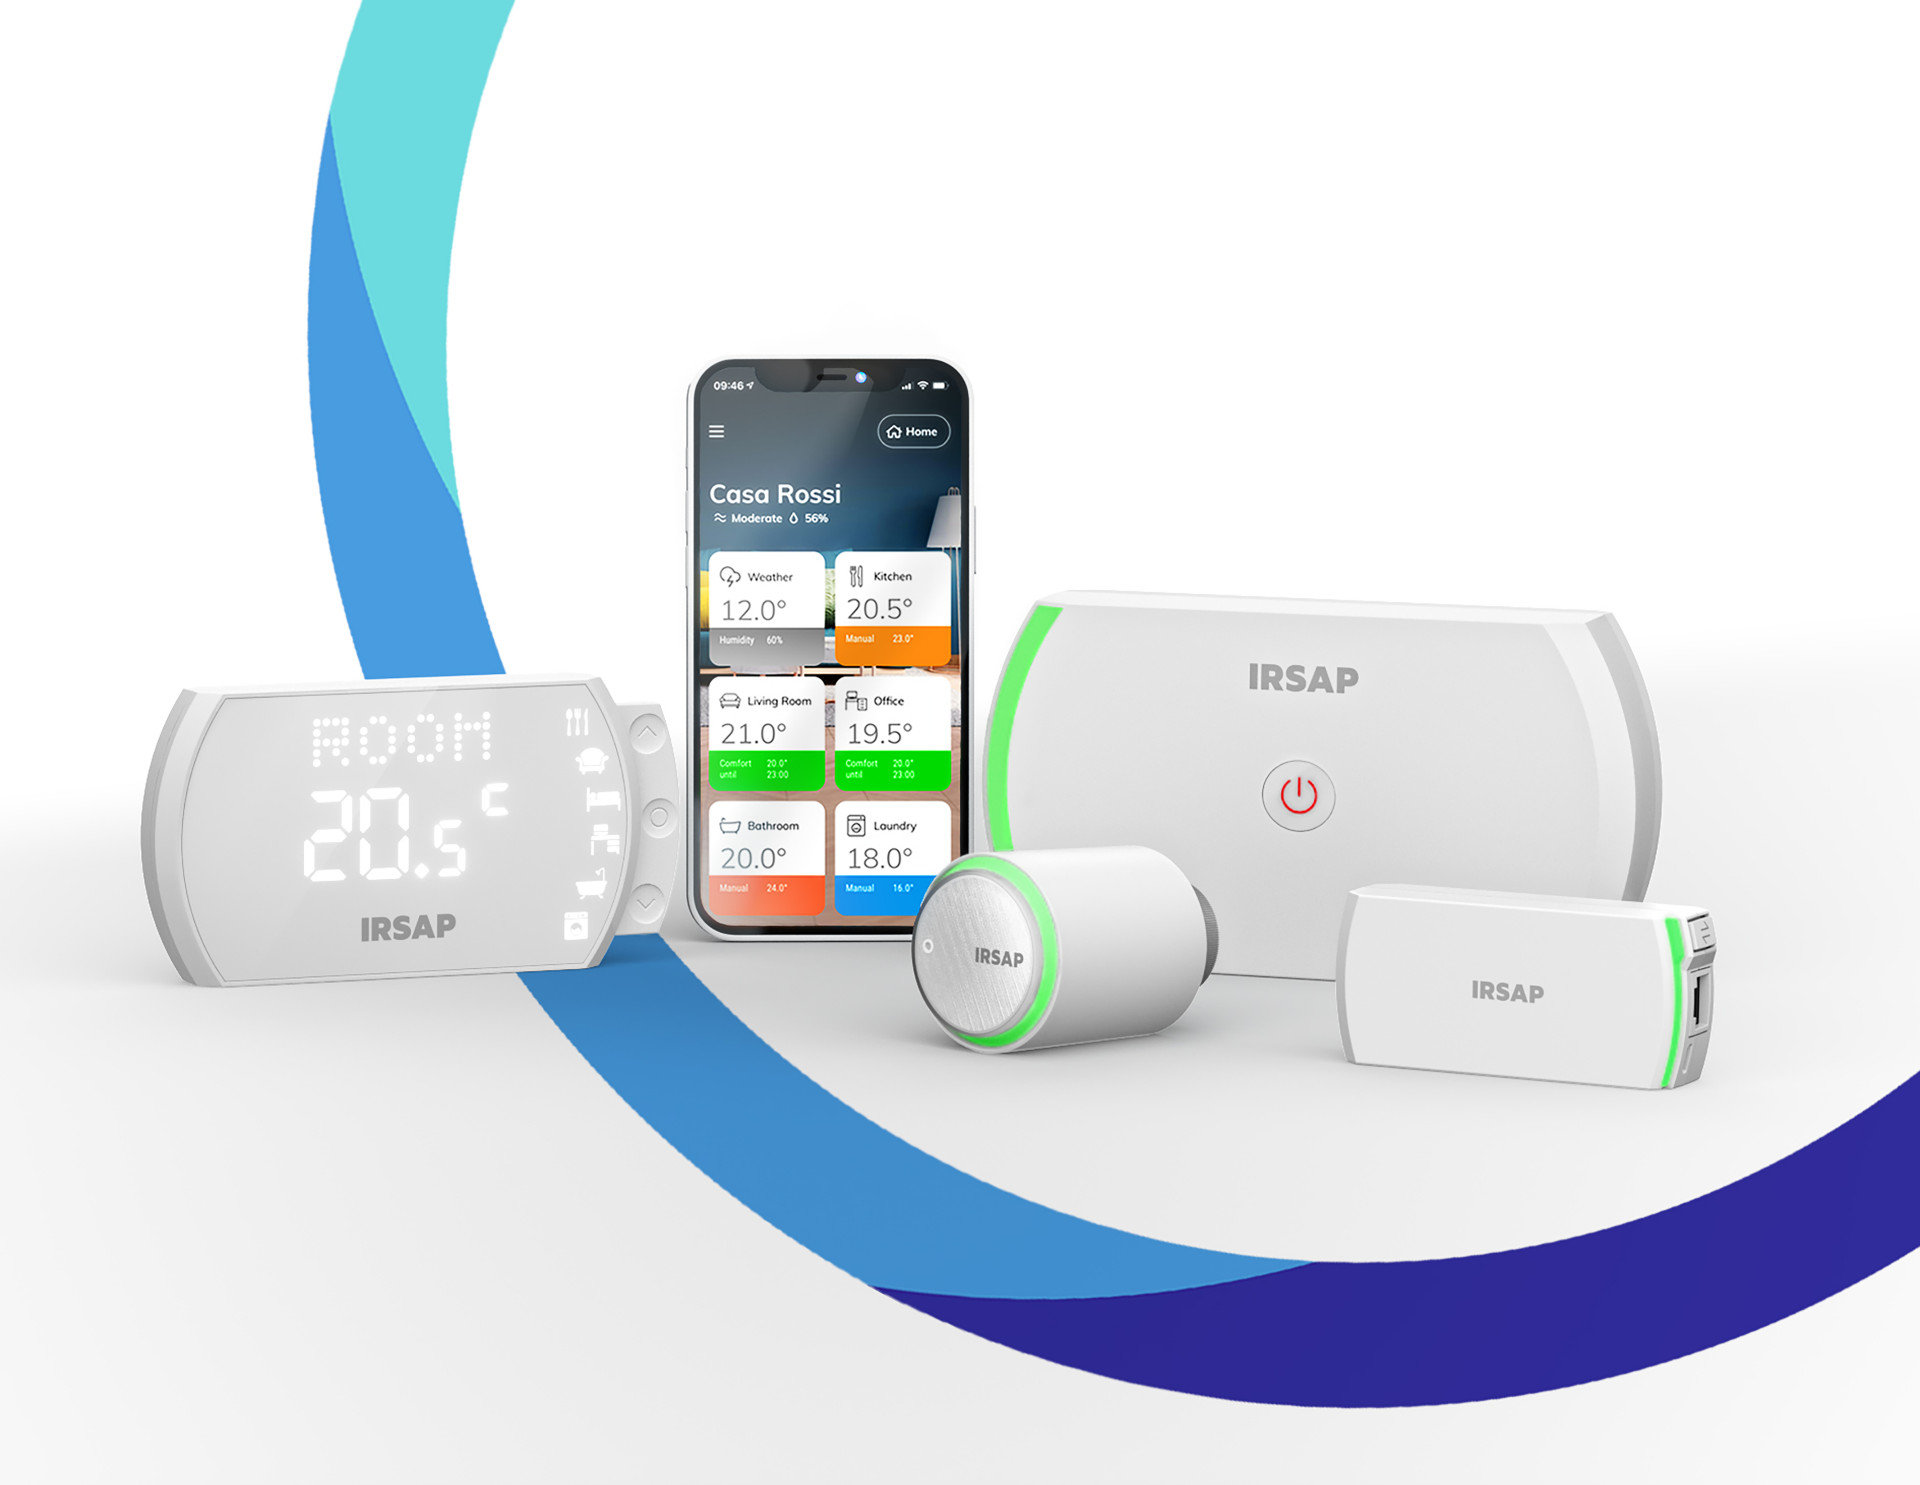
\includegraphics[width=11cm]{img/now.jpeg}
    \caption{Sistema IRSAP NOW per impianti idraulici}
    \label{fig:dispositivi_now}
\end{figure}

Una delle difficoltà attuali è l'impossibilità di andare a testare in maniera isolata i
dispositivi \Gls{rf} e l'unità centrale.

Ad esempio per validare una nuova versione \gls{firmware} della \acrshort{cu} è necessario avere a disposizione tanti dispositivi quanti
ne supporta al massimo il sistema, ovvero 48, un numero che rende molto complessa anche a
livello logistico l'operazione (si pensi ad es. solo al fatto che questi dispositivi funzionano a
batterie che dovrebbero essere continuamente mantenute cariche).

Si potrebbe quindi, mediante un'interfaccia radio opportunamente tarata sulle frequenze usate
dal sistema, andare a simulare i dispositivi lato software, consentendo con un'unica interfaccia
radio di simulare tutti i 48 dispositivi senza fisicamente averli in ufficio.

Oltre a ciò in questo progetto si può porsi anche ad un livello più basso: l'unità
centrale contiene due microcontrollori (e di conseguenza due \gls{firmware}) che comunicano fra di
loro mediante un protocollo seriale (su interfaccia \acrshort{uart}). Uno integra il ricetrasmettitore
a radiofrequenza ed è deputato a gestire la comunicazione con i dispositivi
finali, l'altro invece implementa tutte le logiche di funzionamento incluso l'interfacciamento
con il cloud, che avviene tramite porta ethernet.

Si potrebbe quindi andare a testare i due \gls{firmware} in maniera isolata l'uno dall'altro,
andando a simulare sempre tramite software la controparte mancante. Questo evita di dover
testare tutto i sistema, in particolare la parte \Gls{rf}, quando uno solo dei due software viene
aggiornato. Infatti la parte radio viene aggiornata decisamente più di rado rispetto alla
gestione delle logiche di funzionamento, ma è la più dispendiosa in termini di tempo da testare
(anche perché gestendo a livello fisico la comunicazione \Gls{rf}, in linea teorica, ogni volta andrebbero
rieseguiti i test di laboratorio per assicurarsi che i parametri radio restino nei limiti
imposti dalla normativa vigente).

\section{Test di un termostato}

In IOTINGA infine abbiamo altri progetti \gls{firmware} più complessi su cui questa metodologia
di test potrebbe essere applicata. Uno su tutti il progetto \acrfull{yat},
un cronotermostato \Gls{wifi} in grado di comunicare con la caldaia su bus \Gls{opentherm}, ma
che in futuro verrà prodotto anche in versione \Gls{modbus}.

La peculiarità di questo progetto è il fatto che è prevista l'interazione fra più
termostati mediante \Gls{ble} in modalità Long Range. In questo modo
si può gestire un impianto multizona, in cui vi è uno \acrshort{yat} \textit{master} (alimentato
dalla rete) che mantiene la connessione verso il \gls{cloud} e la comunicazione
con gli altri \acrshort{yat} \textit{slave}, che possono essere alimentati a batteria
in quanto non necessitano di una costante connessione con la rete.

Altra caratteristica dello \acrshort{yat} è un'interfaccia utente (\acrshort{hmi})
locale completa, che utilizza un display a matrice in bianco e nero (o in modelli
futuri a colori TFT) e dei pulsanti capacitivi per navigare nei vari menù. Anche
qui la sfida è riuscire a testare anche l'interfaccia utente in maniera più o meno
automatizzata. Si potrebbe ad esempio escludere completamente il display e verificare
tramite interfacciamento \Gls{spi} che il microcontrollore arrivi a scrivere i dati correttamente
nella memoria video dello schermo.

Come negli scenari visti fin ora anche qui abbiamo una possibilità di gestire configurazioni
differenti, unita al fatto che questo dispositivo verrà venduto anche in modalità ``white label'',
ossia ogni produttore potrà scegliere di andare a personalizzare alcuni aspetti e quindi
avere un \gls{firmware} differente dagli altri. Consegue quindi che ad una modifica potrebbe
corrispondere un numero elevato di binari differenti da testare, uno per cliente, e
ancora la necessità di effettuare dei test automatizzati per garantire la qualità di
quanto finisce in mano ai clienti.

\section{Ringraziamenti}

Ringrazio IOTINGA s.r.l, ed in particolare Matteo e Simone, per questi 3 anni di
lavoro assieme, dove ho potuto sperimentare e migliorare la mia conoscenza su un
numero di tecnologie ed ambiti che è impossibile elencare in un paragrafo.

Ringrazio IRSAP s.p.a., ed in particolare Marco, Leandro, Daniele, Mario, e tutto il team
di \Gls{now} con cui ho potuto lavorare assieme in questi ultimi anni per realizzare
quanto si è visto solo in piccola parte in questo documento.

\appendix

\chapter{Implementazione casi di test}
\section{\nameref{section:test_pairing}}
\label{section:impl_test_pairing}
\inputminted[]{python3}{src/test_pairing.py}

\section{\nameref{section:test_downgrade}}
\label{section:impl_test_downgrade}
\inputminted[]{python3}{src/test_downgrade.py}

\section{\nameref{section:test_ota}}
\label{section:impl_test_ota}
\inputminted[]{python3}{src/test_ota.py}

\section{\nameref{section:test_factory_reset}}
\label{section:impl_test_factory_reset}
\inputminted[]{python3}{src/test_factory_reset.py}

\section{\nameref{section:test_factory_reset_unbounded}}
\label{section:impl_test_factory_reset_unbounded}
\inputminted[]{python3}{src/test_factory_reset_unbounded.py}

\section{\nameref{section:test_thermoregulation}}
\label{section:impl_test_thermoregulation}
\inputminted[]{python3}{src/test_thermoregulation.py}

\section{\nameref{section:test_standby}}
\label{section:impl_test_standby}
\inputminted[]{python3}{src/test_standby.py}

\section{\nameref{section:test_offline_working}}
\label{section:impl_test_offline_working}
\inputminted[]{python3}{src/test_offline_working.py}

\clearpage

\printglossary
\printglossary[type=\acronymtype]

\end{document}
